\documentclass[12pt]{uthesis-v12}  %---> DO NOT ALTER THIS COMMAND

\usepackage{graphicx}
\usepackage{amssymb}
\usepackage{algorithm2e}
\usepackage{algpseudocode}

\begin{document} %---> %---> %---> %---> DO NOT ALTER THIS COMMAND
%--------+----------------------------------------------------------+
%        |  \title{}                                    (REQUIRED)  |
%        |  \author{}                                   (REQUIRED)  |
%        |                                                          |
%        |  See section 3.1 of "Read_Me_First_(v12).pdf"            |
%        |                                                          |
%        |  Also see section 2.2 of above "Read Me" file for the    |
%        |  proper use of the invisible tilde ("~") character when  |
%        |  entering a middle initial in the \author command.       |
%        +----------------------------------------------------------+

\title{A Context-Aware Approach
       \protect\\ to Android Memory Management}
       
% Alternatively, A User-Centric Approach to Android Memory Management

\author{Srinivas Muthu}

%--------+----------------------------------------------------------+
%        |  \copyrightpage{}                            (REQUIRED)  |
%        |                                                          |
%        |  See section 3.2 of "Read_Me_First_(v12).pdf"            |
%        |                                                          |
%        |  1) You must enter either "yes" or "no" in this          |
%        |      command.  Inputting "yes" produces a copyright      |
%        |      notification page as the second page and inputting  |
%        |      "no" produces a blank second page.                  |
%        |  2) Input to this command is case sensitive.             |
%        |  3) Default: the "yes" option.                           |
%        +----------------------------------------------------------+

\copyrightpage{yes}

%--------+----------------------------------------------------------+
%        |  \mydocument{}                               (REQUIRED)  |
%        |                                                          |
%        |  See section 3.3 of "Read_Me_First_(v12).pdf"            |
%        |                                                          |
%        |  1) Input to this command is limited to the following    |
%        |     three options: a) Dissertation                       |
%        |                    b) Thesis                             |
%        |                    c) Project                            |
%        |  2) Input to this command is case-sensitive.             |
%        +----------------------------------------------------------+

\mydocument{Thesis}

%--------+----------------------------------------------------------+
%        |  \degree{}{}                                 (REQUIRED)  |
%        |                                                          |
%        |  See section 3.4 of "Read_Me_First_(v12).pdf"            |
%        |                                                          |
%        |  You need to provide two distinct inputs into this       |
%        |  command:                                                |
%        |     1) In the first set of braces you need to specify    |
%        |        the *exact* degree you will receive. Some         |
%        |        examples are: -) Masters of Arts                  |
%        |                      -) Masters of Science               |
%        |                      -) Doctor of Philosophy             |
%        |     2) In the second set of braces you need to state the |
%        |        *specific* discipline or area for that degree     |
%        |        (e.g., Economics, Education, Engineering, etc.).  |
%        |  Students should consult their advisor if they have any  |
%        |  questions about this information.                       |
%        +----------------------------------------------------------+

\degree{Masters of Science}{Engineering}

%--------+----------------------------------------------------------+
%        |  \conferraldate{}{}                          (REQUIRED)  |
%        |                                                          |
%        |  See section 3.5 of "Read_Me_First_(v12).pdf"            |
%        |                                                          |
%        |  In the two set of braces enter the month and then the   |
%        |  year your degree will be *conferred* by the university. |
%        +----------------------------------------------------------+

\conferraldate{December}{2015}

%--------+----------------------------------------------------------+
%        |  \advisor{}                                  (REQUIRED)  |
%        |                                                          |
%        |  See section 3.6.2 of "Read_Me_First_(v12).pdf"          |
%        |                                                          |
%        |  1) Also see section 2.2 of "Read_Me_First_(v12).pdf"    |
%        |     for the proper use of the invisible tilde ("~")      |
%        |     character when entering a middle initial or the      |
%        |     abbreviation of an academic title (e.g., Dr.) in     |
%        |     the \advisor{} command.                              |
%        |  2) Also see section 3.6.1. for consistent presentation  |
%        |     of title page signature lines.                       |
%        +----------------------------------------------------------+

\advisor{Dr.~Jackson Carvalho}

%--------+----------------------------------------------------------+
%        |  Committee Member Signature Commands         (OPTIONAL)  |
%        |                                                          |
%        |  See section 3.6.3 of "Read_Me_First_(v12).pdf"          |
%        |                                                          |
%        |  1) Use the commands below to provide signature lines    |
%        |     for your "other" committee members;                  |
%        |        --> you must list your other committee members    |
%        |            in alphabetic order by last name              |
%        |        --> to do this, use the commands below in the     |
%        |            order presented below.                        |
%        |  2) You can choose to include none, some, or all of the  |
%        |     "XXXmember" commands below --- based on the number   |
%        |     committee members you have; simply delete (or        |
%        |     comment-out) any of the commands below that are not  |
%        |     needed.                                              |
%        |  3) Do not include the name of your committee chair or   |
%        |     the Graduate Dean in the commands listed below.      |
%        |     Their signature lines are generated by the           |
%        |     \advisor{} and \graduatedean{}{} commands.           |
%        |  4) You cannot use any of the commands below more than   |
%        |     once. (For details on this issue, see section 3.6.3  |
%        |     of "Read_Me_First_(v12).pdf".)                       |
%        |  5) Also see section 2.2 of "Read_Me_First_(v12).pdf"    |
%        |     for the proper use of the invisible tilde ("~")      |
%        |     character when entering a middle initial or the      |
%        |     abbreviation of an academic title (e.g., Dr.) in     |
%        |     the commands below.                                  |
%        |  6) See section 3.6.1. for consistent presentation of    |
%        |     title page signature lines.                          |
%        |                                                          |
%        |  I know I shouldn't have to say this, but enough         |
%        |  students over the years have made the same mistake      |
%        |  that I'm forced to state:                               |
%        |                                                          |
%        |      THE NAMES USED IN THE FOLLOWING COMMANDS ARE        |
%        |      SILLY NAMES I'VE USED AS EXAMPLES ONLY.  THEY       |
%        |      ARE NOT THE ACTUAL NAMES OF YOUR COMMITTEE          |
%        |      MEMBERS.  REPLACE THE SILLY NAMES BELOW WITH        |
%        |      THE NAMES OF YOUR ACTUAL COMMITTEE MEMBERS.         |
%        |                                                          |
%        +----------------------------------------------------------+

  \secondmember{Dr.~Mansoor Alam}
   \thirdmember{Dr.~Henry Ledgard}

%--------+----------------------------------------------------------+
%        |  \graduatedean{}{}                           (REQUIRED)  |
%        |                                                          |
%        |  See section 3.6.4 of "Read_Me_First_(v12).pdf"          |
%        |                                                          |
%        |  1) THE NAME AND TITLE PROVIDED BELOW ARE THOSE OF THE   |
%        |     ACTUAL GRADUATE DEAN AT THE TIME THIS DOCUMENT WAS   |
%        |     CONSTRUCTED (January 2012). Contact the Graduate     |
%        |     College to determine whether this information is     |
%        |     correct at the time you submit your document.        |
%        |  2) Section 2.2 of "Read_Me_First_(v12).pdf" describes   |
%        |     the proper use of the invisible tilde ("~")          |
%        |     character when entering a middle initial or the      |
%        |     abbreviation of an academic title (e.g., Dr.) in     |
%        |     the \graduatedean{} command.                         |
%        |  3) See section 3.6.1. for consistent presentation of    |
%        |     title page signature lines.                          |
%        +----------------------------------------------------------+

\graduatedean{Dr.~Patricia R.~Komuniecki}{Dean}

%--------+----------------------------------------------------------+
%        |  \maketitle                                  (REQUIRED)  |
%        |                                                          |
%        |  See section 3.7 of "Read_Me_First_(v12).pdf"            |
%        |                                                          |
%        |  This is a required LaTeX command; to be brief, bad      |
%        |  things will happen if this command is not included      |
%        |  in your document at this particular location.           |
%        +----------------------------------------------------------+

\maketitle  %---->  ----->  ---->  ---->   DO NOT ALTER THIS COMMAND

%--------+----------------------------------------------------------+
%        |  Abstract Page Environment                   (REQUIRED)  |
%        |                                                          |
%        |  See section 3.8 of "Read_Me_First_(v12).pdf"            |
%        +----------------------------------------------------------+

\begin{abstractpage}
	smartphones are ubiquitous and operate in diverse environments. Hence, they are well suited to utilize contextual information in enhancing the behavior of their applications. However, the potential of context analysis is not fully utilized by Android devices. The Android operating system caches the processes of recently-used applications in memory, so that they can be loaded quickly should the user request them again. We postulate that incorporating context information can improve this caching scheme. As a proof of concept, we setup an experiment comprising of twenty volunteers (Android smartphone users) and compared the cache hit ratios of the default scheme with a default-context hybrid scheme. This hybrid scheme incorporated information from the user's calendar in determining which processes were cached.  To accomplish this task, each volunteer installed an Android application that parses their Calendar for contextual clues and generates a list of applications that the user is likely to use. This list is then combined with the default list (that Android generates through recency of usage) to determine the cache hit ratios of the hybrid scheme. Finally, we use the data collected from the experiment to show why the hybrid scheme is more efficient and on a broader level, that context analysis is beneficial in enhancing the user experience.        
\end{abstractpage}

%--------+----------------------------------------------------------+
%        |  Dedication Page Environment                 (OPTIONAL)  |
%        |                                                          |
%        |  See section 3.9 of "Read_Me_First_(v12).pdf"            |
%        |                                                          |
%        |  If both a dedication page and an acknowledgements page  |
%        |  are included in the document, the dedication page must  |
%        |  proceed the acknowledgements page.                      |
%        +----------------------------------------------------------+

\begin{dedication}
\noindent To my parents who have always put my needs ahead of theirs.
\end{dedication}

%--------+----------------------------------------------------------+
%        |  Acknowledgments Page Environment            (OPTIONAL)  |
%        |                                                          |
%        |  See section 3.10 of "Read_Me_First_(v12).pdf"           |
%        |                                                          |
%        |  If both a dedication page and an acknowledgements page  |
%        |  are included in the document, the dedication page must  |
%        |  proceed the acknowledgements page.                      |
%        +----------------------------------------------------------+

\begin{acknowledgments}
\noindent First and foremost, I would like to thank Dr.~Jackson Carvalho for mentoring me throughout my time here at UT. Without his guidance, I would not be half the student I am today. I would like to thank Dr.~Mansoor Alam for believing in me and offering me tuition scholarship to pursue graduate studies, here at UT. I would like to thank Dr.~Lawrence Thomas for being an exemplary professor and his words of wisdom have always guided me in tough times.\\\\I am grateful to Dr.~Henry Ledgard for taking the time to be on my committee and mentoring me during my freshman year. I would like to thank Dr.~Donald White and his students for helping me with data collection, design and representation. It was nothing short of a privilege to work with Dr.~White and his students. I would like to thank Dean Nagi G.~Naganathan for employing me and guiding me over the course of my time in graduate school. Without the help of research volunteers, this work would not have been possible and I would like to convey my gratitude to every volunteer that signed up for the experiment.\\\\
I would like to thank all my friends and family for supporting me throughout my time here at UT but I would like to especially mention Sandy Stewart for everything she has done for me. This page is not enough to expound on the details but it suffices to say I would not be here without her and she is like a second mother to me.  
\end{acknowledgments}

%--------+----------------------------------------------------------+
%        |  \tableofcontents                            (REQUIRED)  |
%        |  \listoftables                            (CONDITIONAL)  |
%        |  \listoffigures                           (CONDITIONAL)  |
%        |                                                          |
%        |  See sections 3.11 & 3.12 of "Read_Me_First_(v12).pdf"   |
%        |                                                          |
%        |  1) You must include the \tableofcontents command in     |
%        |     your document: the UT Manual requires every          |
%        |     dissertation/thesis to have a detailed table of      |
%        |     contents.                                            |
%        |  2) Including the \listoftables and \listoffigures       |
%        |     commands is "conditional."  See sections 3.12 of     |
%        |     "Read_Me_First_(v12).pdf" for additional details.    |
%        +----------------------------------------------------------+

\tableofcontents  %----->  ----->  ---->  DO NOT ALTER THIS COMMAND
\listoffigures

%--------+----------------------------------------------------------+
%        |  \captionformat{}                            (REQUIRED)  |
%        |                                                          |
%        |  See section 3.12.2 of "Read_Me_First_(v12).pdf"         |
%        |                                                          |
%        |  1) You are required to choose between the "hang" or     |
%        |     "align" option for this command.                     |
%        |  2) Input to this command is case sensitive.             |
%        |  3) Default: ``hang'' option.                            |
%        +----------------------------------------------------------+

\captionformat{hang}

%--------+----------------------------------------------------------+
%        |  List of Abbreviations Environment           (OPTIONAL)  |
%        |                                                          |
%        |  See section 3.13 of "Read_Me_First_(v12).pdf"           |
%        |                                                          |
%        |  1) This is an optional section; consult your advisor    |
%        |     to determine whether you need/want to include this   |
%        |     section in your document.                            |
%        |  2) If you do not want a List of Abbreviations simply    |
%        |     delete the material below (and these instructions).  |
%        |  3) If you do want a List of Abbreviations simply        |
%        |     replace the silly material below with the            |
%        |     information relevant to your document.               |
%        |     a. Within the "listofabbreviations" environment      |
%        |        below you must use a separate \abbreviation{}{}   |
%        |        command for each entry in your List of            |
%        |        Abbreviations.                                    |
%        |     b. As the examples below demonstrate, the            |
%        |        information within the first set of braces is     |
%        |        the abbreviation and the information in the       |
%        |        second set of braces is the definition of that    |
%        |        abbreviation.                                     |
%        +----------------------------------------------------------+

\begin{listofabbreviations}

 \abbreviation{RAM}{Random Access Memory}
 \abbreviation{CHR}{Cache Hit Ratio}
 \abbreviation{OS}{Operating System}
 \abbreviation{AOSP}{Android Open Source Project}
 \abbreviation{APK}{Android Package} 
 \abbreviation{APMD}{Android Powered Mobile Device}
 \abbreviation{CBP}{Cached Background Process} 
 \abbreviation{OEM}{Original Equipment Manufacturer}
 \abbreviation{ADB}{Android Debug Bridge}
 \abbreviation{UID}{Unique Identifier}
 \abbreviation{OOM}{Out Of Memory}
 \abbreviation{API}{Application Programming Interface} 
 \abbreviation{USA}{United States of America} 
 \abbreviation{UI}{User Interface}
 \abbreviation{PPMCC}{Pearson Product Moment Correlation Coefficient}
 \abbreviation{CI}{Confidence Interval}

\end{listofabbreviations}

%--------+----------------------------------------------------------+
%        |  List of Symbols Environment                 (OPTIONAL)  |
%        |                                                          |
%        |  See section 3.14 of "Read_Me_First_(v12).pdf"           |
%        |                                                          |
%        |  1) This is an optional section; consult your advisor    |
%        |     to determine whether you need/want to include this   |
%        |     section in your document.                            |
%        |  2) If you do not want a List of Symbols simply delete   |
%        |     the material below (and these instructions).         |
%        |  3) If you do want a List of Symbols simply replace the  |
%        |     silly material below with the information relevant   |
%        |     to your document.                                    |
%        |       a. Within the "listofsymbols" environment below    |
%        |          you must use a separate \emblem{}{} command     |
%        |          for each entry in your List of Symbols.         |
%        |       b. As the examples below show, insert your symbol  |
%        |          within the first set of braces in the           |
%        |          \emblem{}{} command, and its definition within  |
%        |          the second set of braces.                       |
%        |       c. Use the \emblemskip command to insert a blank   |
%        |          line between different categories of symbols:   |
%        |          -) such additional spacing is required between  |
%        |             different categories of symbols;             |
%        |          -) see "Read_Me_First_(v12).pdf" for details.   |
%        +----------------------------------------------------------+

\begin{listofsymbols}

 \emblem{\checkmark}{Represents a check mark indicating that a particular item has been checked or in a different context, whether the checked item is correct}
 
% \emblem{$\ddagger$}{the degree to which the flayrod has gone out of
%                    skew on tredel}
%\emblem{$\triangle$}{the ratio of the M2 monetary aggregate to the
%                    Monetary Base}
%
%       \emblemskip
%
%  \emblem{$\alpha$}{angle of rotation around internal rotation axis}
%   \emblem{$\beta$}{the number of people named ``Bob''}
%
%       \emblemskip
%
%         \emblem{Q}{Tobin's q; the ratio of the market value of
%                    installed capital to the replacement cost of
%                    capital}
%         \emblem{Y}{Gross Domestic Product (adjusted for inflation)}

\end{listofsymbols}

%--------+----------------------------------------------------------+
%        |  Preface Environment                         (OPTIONAL)  |
%        |                                                          |
%        |  See section 3.15 of "Read_Me_First_(v12).pdf"           |
%        +----------------------------------------------------------+

\begin{preface}
This thesis is original, unpublished, independent work by the author, Srinivas Muthu under the tutelage of Dr.~Jackson Carvalho.
\end{preface}

%XXXXXXXXXXXXXXXXXXXXXXXXXXXXXXXXXXXXXXXXXXXXXXXXXXXXXXXXXXXXXXXXXXXX
%XXXXXXXXXXXXXXXXXXXXXXXXXXXXXXXXXXXXXXXXXXXXXXXXXXXXXXXXXXXXXXXXXXXX
%XXXXXXXXXXXXXXXXXXXXXXXXXXXXXXXXXXXXXXXXXXXXXXXXXXXXXXXXXXXXXXXXXXXX
%XXXXXXXXXXXXXXXXXXXXXXXXXXXXXXXXXXXXXXXXXXXXXXXXXXXXXXXXXXXXXXXXXXXX

%--------+----------------------------------------------------------+
%        |  \makebody                                   (REQUIRED)  |
%        |                                                          |
%        |  See section 3.16 of "Read_Me_First_(v12).pdf"           |
%        |                                                          |
%        |  This is a *required* UThesis command; again, bad        |
%        |  things will happen if this command is not included in   |
%        |  your document at this particular location --- see the   |
%        |  file "Read_Me_First_(v12).pdf" for details.             |
%        +----------------------------------------------------------+

\makebody   %------->  ------->  ------->  DO NOT ALTER THIS COMMAND

%XXXXXXXXXXXXXXXXXXXXXXXXXXXXXXXXXXXXXXXXXXXXXXXXXXXXXXXXXXXXXXXXXXXX
%XXXXXXXXXXXXXXXXXXXXXXXXXXXXXXXXXXXXXXXXXXXXXXXXXXXXXXXXXXXXXXXXXXXX
%XXXXXXXXXXXXXXXXXXXXXXXXXXXXXXXXXXXXXXXXXXXXXXXXXXXXXXXXXXXXXXXXXXXX
%XXXXXXXXXXXXXXXXXXXXXXXXXXXXXXXXXXXXXXXXXXXXXXXXXXXXXXXXXXXXXXXXXXXX

%--------+----------------------------------------------------------+
%        |  \chapter{}                                  (REQUIRED)  |
%        |                                                          |
%        |  See section 3.17 of "Read_Me_First_(v12).pdf"           |
%        |                                                          |
%        |  For guidance on using the commands \chapter{},          |
%        |  \section{}, \subsection{}, \subsubsection{}, etc., see  |
%        |  Leslie Lamport's "LaTeX: A Document Preparation         |
%        |  System." Addison Wesley: Reading Massachusetts, 1985.   |
%        +----------------------------------------------------------+

\chapter{Introduction}
	
	\section{Problem}
		With the advent of increase in the amount of RAM (Random Access memory) available in Android smartphones, there is a case to be made that this additional memory availability can be put to better use. By default, every Android application runs in its own Linux process [34]. When a smartphone that runs on Android is active, the RAM contains all the active processes [3] and services [2]. In addition, it also contains cached background processes. These processes are kept in memory so that in the event the user clicks any of the corresponding applications, they can be loaded onto the screen quickly, thereby enhancing the user experience. Consequently, it is in Android's best interests to maximize the chances of the user requesting one of these applications. Currently, Android uses recency of usage to determine which applications get cached. To elaborate, the most recently used applications are cached as cached background processes. Therefore, the problem at hand is determining whether there is a better caching scheme and whether contextual information can be influential in such a scheme.
		
	\section{Proposed Solution}		
		We postulate that incorporating context information can lead to a better caching scheme. In our case we utilize context by looking into the user's calendar to try and predict which applications the user is likely to use in the near future. This leads to three possible caching schemes:
		
		\begin{itemize}
			\item Default Scheme (based on caching recently used applications)
			\item Context Scheme (based on caching applications predicted by reading the user's calendar)
			\item Default-Context Hybrid Scheme (based on caching applications from both groups)
		\end{itemize}
		
		We need to measure the efficiency of each scheme in order to determine the best one. To accomplish this task, we setup an experiment that comprised of twenty android smartphone users, to measure the cache hit ratios of each scheme. We developed an Android application that parsed the user's calendar and generated a list of applications likely to be used by the user. Additionally, it collected the basic cache metrics (cache hit, cache miss, cache hit ratio) for each scheme. We thoroughly analyze the data collected and demonstrate the superiority of the default-context hybrid scheme.  
		
		\subsection{Assumptions}	
			We have made the following assumptions:
			\begin{itemize}
				\item For the purpose of this thesis, the user's context is obtained through reading the user's calendar.
				\item All the research volunteers own an Android smartphone that operates at API (Application Programming Interface) Level 21 and above [41].
				\item Each volunteer authorized the application to access their calendar.
			\end{itemize}
			
			Chapter 4 elaborates on why volunteers require API level 21 and above. Android mandates that the user authorize all permissions for third-party applications to access their data, during installation.
			
	\section{Checking Applications in RAM}
		Every Android smartphone user is capable of checking the processes that currently reside in physical memory. The Application Manager which is part of the Settings application shows a list of running processes and cached background processes. Additionally, it breaks down the composition of RAM usage (Figure 1-1) by the System applications and user installed applications. 
		
		\begin{figure}[h]
			\centering
			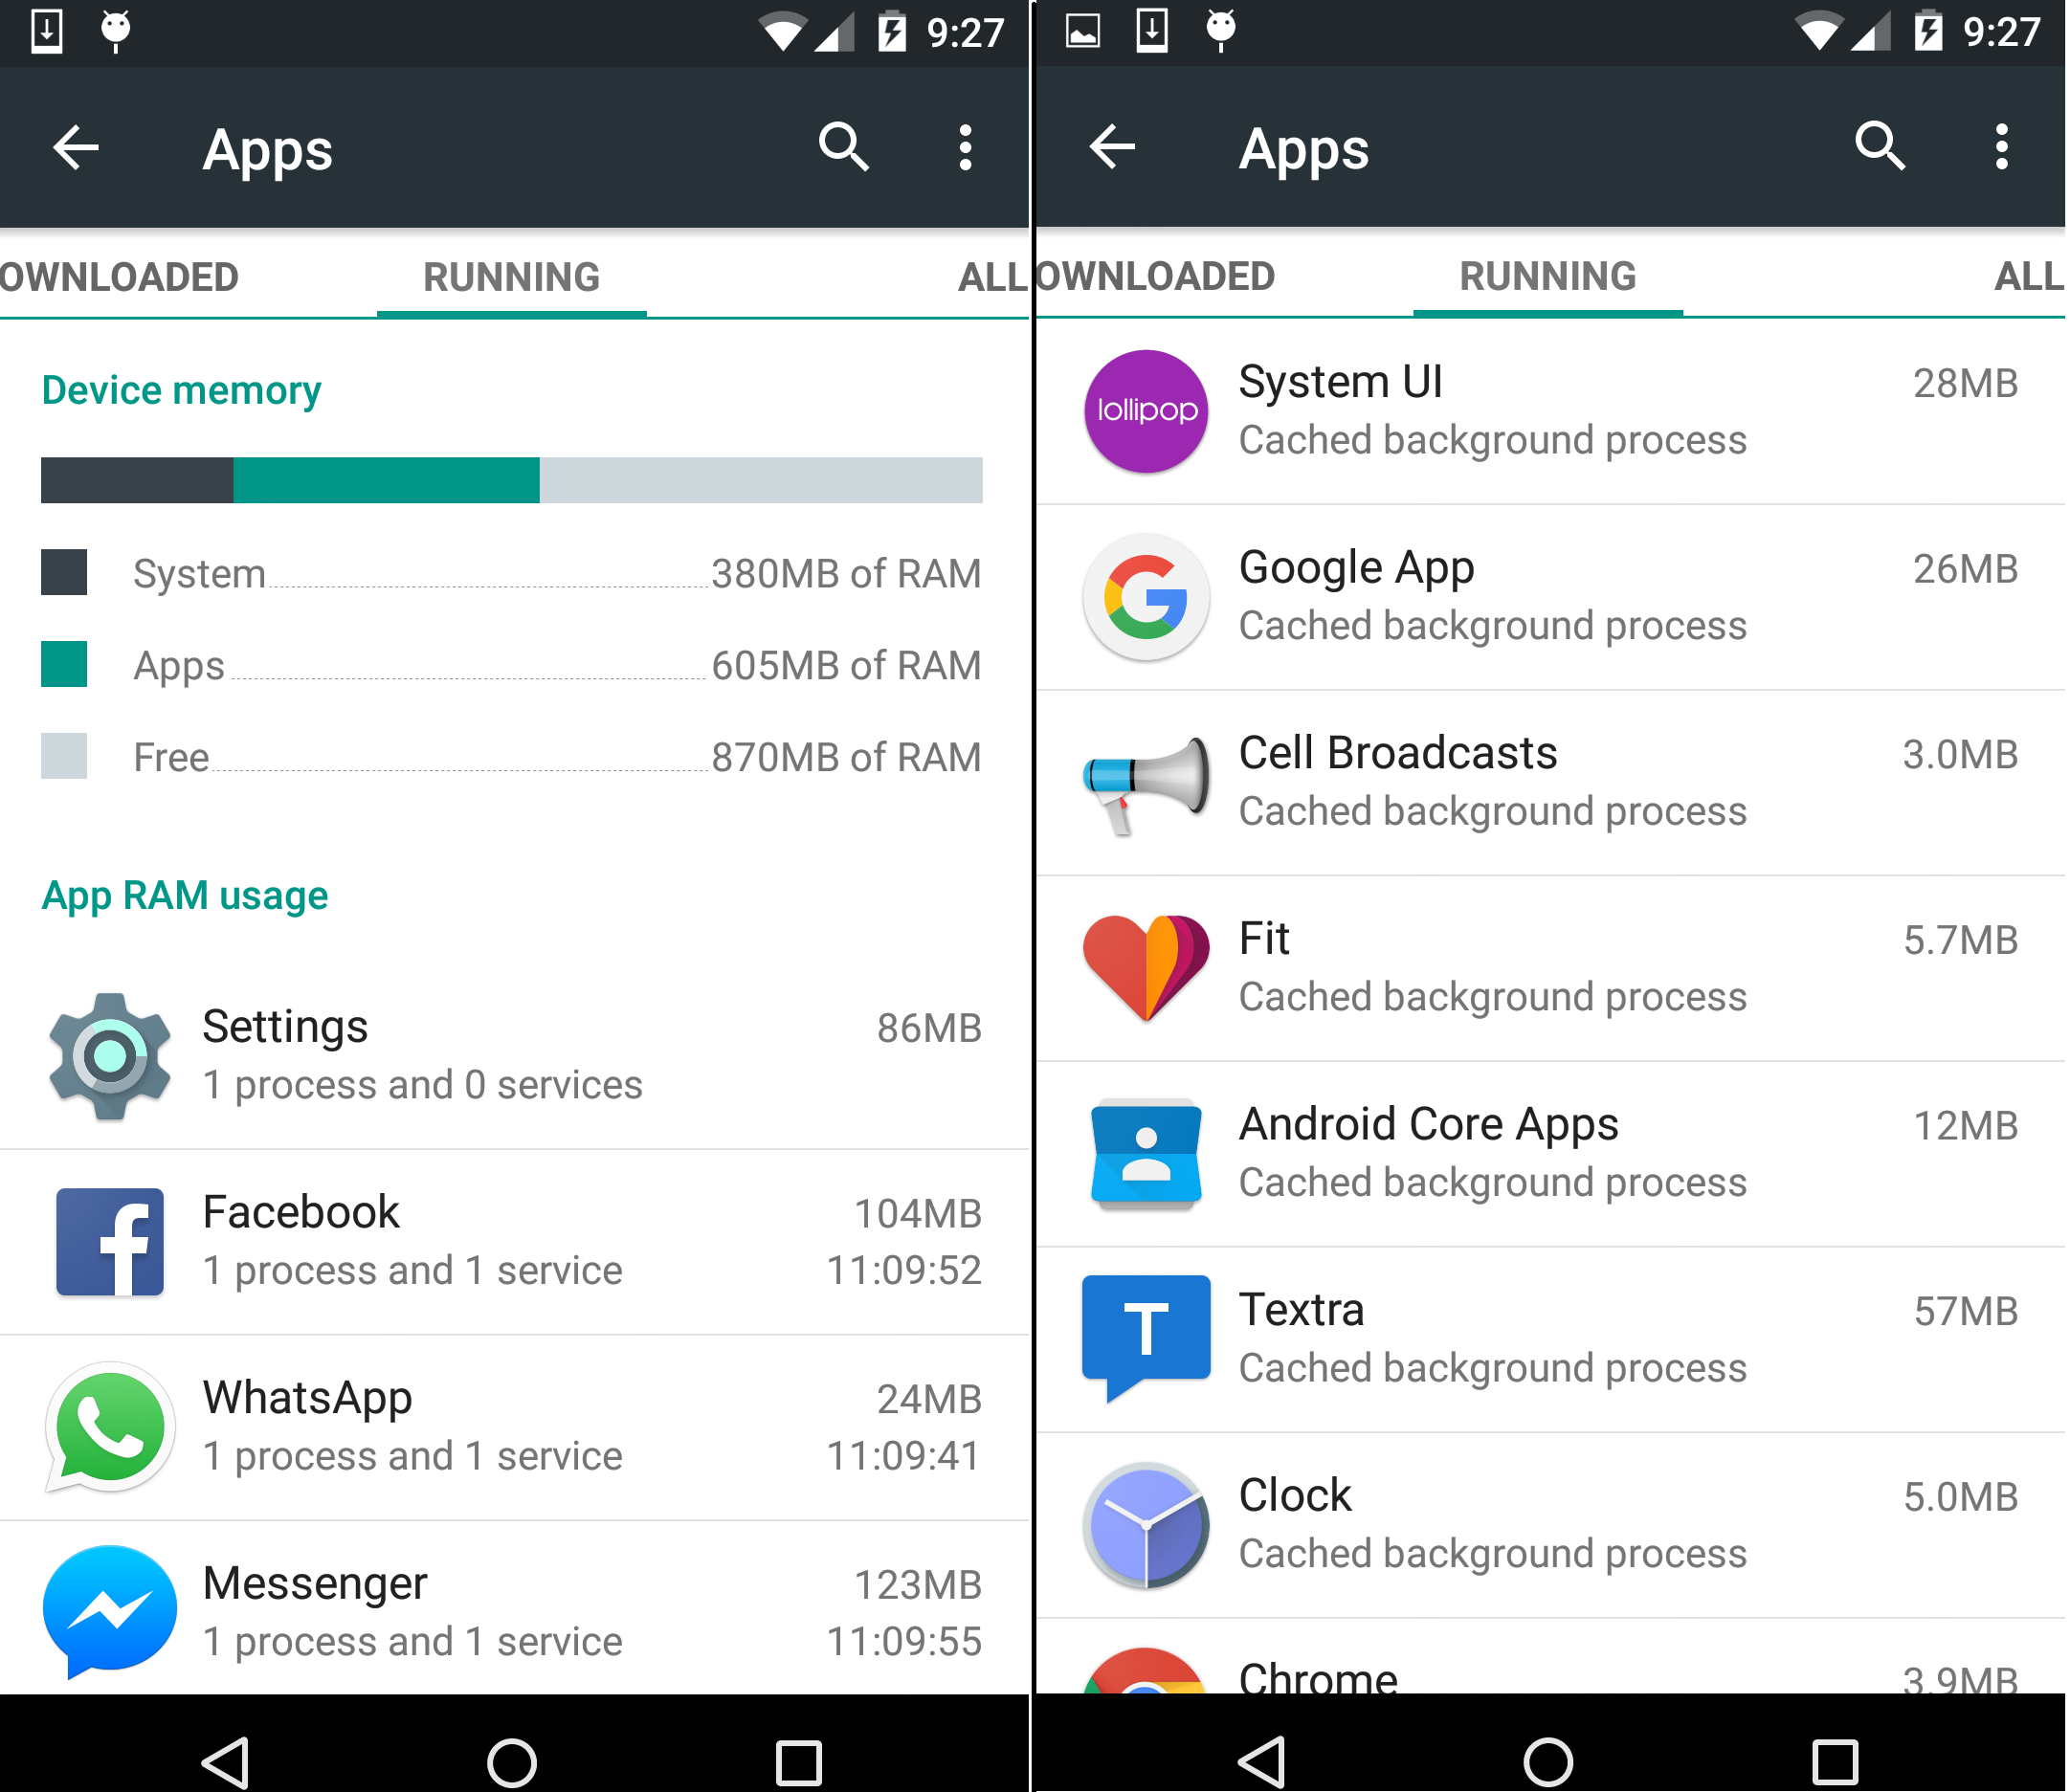
\includegraphics[width = 90mm]{images/runningApps.png}
			\caption[Running Applications and Cached Background Processes]
			{Left - List of Running Applications (Active Processes and Services)\\
				Right - List of Cached Background Processes}
		\end{figure}	

	\section{Organization of Thesis}
		Several works in the past have focused on context-aware applications and ways to observe user behavior patterns. We will explore some these works and how this contextual data was put to use in Chapter 2. In Chapter 3, we will take a look at some of the challenges in collecting cache metrics such as detecting the applications in memory, detecting when the user clicks a new application, whether to approach the problem at the user level or the system level, to list a few. Chapter 4 elaborates on the setup of the experiment and analyzes the design of the application used to collect these metrics. We dive into the data in Chapter 5 and summarize the results. We also investigate how certain supplementary factors could explain the distribution of data. In Chapter 6, we discuss some of the shortcomings of this thesis and conclude the thesis with Chapter 7. Finally, chapter 8 talks about scope for future work and explores some of the possibilities of directly adding to this thesis.  


%				How to Refer to a table, look below:

%[ Insert your text to chapter 1 here.  A pretend example of a silly
%table is provided below (i.e., Table~\ref{SILLY}).~]

%								Table Template


%     \vfill
%     \begin{table}[ht]
%     \caption{A silly glossary for research reports.\label{SILLY}}
%     \begin{center}
%     \begin{tabular}{p{2.75in}|p{2.5in}}
%      \rule[-0.5em]{0pt}{1.75em} \bf When Professors write \ldots
%      & \bf they REALLY mean \ldots \\ \hline\hline
%      %--------+------------------------------------
%      \rule[-0.5em]{0pt}{1.75em} Typical results are shown \ldots
%      & The best results are shown \ldots \\ \hline
%      %--------+------------------------------------
%      \rule[-0.5em]{0pt}{1.75em} It is generally believed that
%      \ldots & A couple of other guys think so too  \\ \hline
%      %--------+------------------------------------
%      \rule[-0.5em]{0pt}{1.75em}Thanks to Al K.~Seltzer for
%      assistance and to I.P. Daly for valuable discussions &
%      Seltzer did the work and Daly explained
%      what it meant \\
%     \end{tabular}
%     \end{center}
%     \end{table}
%     \vfill

%XXXXXXXXXXXXXXXXXXXXXXXXXXXXXXXXXXXXXXXXXXXXXXXXXXXXXXXXXXXXXXXXXXXX
%XXXXXXXXXXXXXXXXXXXXXXXXXXXXXXXXXXXXXXXXXXXXXXXXXXXXXXXXXXXXXXXXXXXX
%XXXXXXXXXXXXXXXXXXXXXXXXXXXXXXXXXXXXXXXXXXXXXXXXXXXXXXXXXXXXXXXXXXXX
%XXXXXXXXXXXXXXXXXXXXXXXXXXXXXXXXXXXXXXXXXXXXXXXXXXXXXXXXXXXXXXXXXXXX


\chapter{Related Work}
	
	\section{Early Studies in Context-Aware Computing}
		Dey, Abowd and Salber, in their 2001 paper titled {\em A conceptual framework and a toolkit for supporting the rapid prototyping of context-aware applications} laid out the foundation and in many ways a standardized framework for building context-aware applications. When this paper was published, mobile phones were becoming mainstream devices and were no longer confined to the hands of a few. By definition, more people were mobile and the devices they carried with them had the potential to utilize contextual information gathered from the surroundings, in ways that desktops could not do due to their stationary nature. Dey et al. defined context as any information that characterizes a situation related to the interaction between humans, applications and the surrounding environment. They opined that the state of research in context-awareness was inadequate for three main reasons:
		
		\begin{itemize}
			\item The notion of context was ill-defined.
			\item There was a lack of conceptual models and methods to help drive the design of context-aware applications.
			\item No tools were available to jump-start the development of context-aware applications.
		\end{itemize}
		
		 They focused their efforts on the pieces of context that could be inferred automatically from sensors in a physical environment and produced Context Toolkit [6], a conceptual framework that supported the rapid development of context-aware applications. It is important to keep in mind that at the time this paper was published, the notion of what we refer to as a smartphone was non-existent. This is evident from the fact that most APMD (Android Powered Mobile Device)(s) have built-in sensors that measure motion, orientation, and various environmental conditions. These sensors are capable of providing raw data with high precision and accuracy, and are useful in monitoring three-dimensional device movement or positioning, or changes in the ambient environment near a device [7]. These conditions make APMD(s) very suitable for utilizing contextual information and translating that potential into a better user experience. We utilize this feature of APMD(s) to propose ways to improve user experience by incorporating contextual information in managing its physical.		
			
	\section{Context Patterns in Application Usage}
		Several works have attempted to collect user behavior data and they have accomplished this in unique ways. Hannu Verkasalo, in his 2007 paper titled {\em Contextual Patterns in Mobile Service Usage} analyzes how mobile services are used in different contexts [4]. Usage contexts were divided into {\em home, office} and {\em on the move}. A specialized algorithm tracked user's location patterns over a period of time to determine whether the user was at home or at work. Furthermore, changes in location data revealed whether the user was in transit between home and work. There was a correlation between the mobile services requested by the user and the user's physical location, which enabled the algorithm to understand the user's context quite well (Figure 2-1). It was also observed that certain services were requested more during the weekends as opposed to certain others being requested more during the weekdays i.e. days with office hours.  
		
		\begin{figure}[!ht]
			\centering
			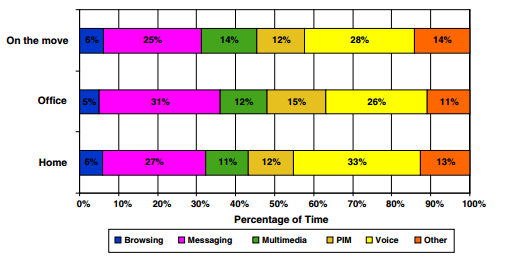
\includegraphics[width = 90mm]{images/appsByTime.png}
			\caption[Mobile Services Requested at Various Times of the Day]
			{By classifying user context into three distinct entities namely {\em home, work} and {\em on the move}, the author managed to infer which services were requested more in a given context. For e.g. Voice services i.e. calling was predominantly requested while the user was at home. This type of information can be very useful.}
		\end{figure}
	
	\section{Context Phone}
		Mika Raento, Antti Oulasvirta, Renaud Petit, and Hannu Toivonen, in their paper titled {\em ContextPhone: A Prototyping Platform for Context-Aware Mobile Applications} proposed that mobile phones are well suited for context aware computing due to an intimate relationship between the user and the phone [5]. Their primary goal was to provide context as a resource and in order to accomplish that, developed a {\em ContextPhone} which comprised of four components (Figure 2-2):
		
		\begin{itemize}
			\item Sensors that acquire contextual data (such as location data from GPS)
			\item Communication services (such as SMS, MMS to list a few)
			\item Customizable Applications (that can replace existing applications)
			\item System Services (such as background services for error logging)
		\end{itemize}
		
		
		\begin{figure}[!ht]
			\centering
			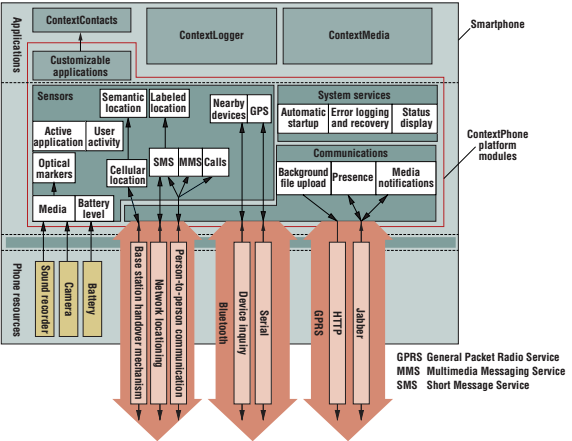
\includegraphics[width = 90mm]{images/contextPhone.png}
			\caption[Context Phone]
			{The ContextPhone platform; Four interconnected components — sensors, system services, communication services, and customizable applications — facilitate communication with the outside world.}
		\end{figure}
		
		It is important to observe that this paper came out in 2005, two years before the first version of Android was even launched. Yet, their fundamental point of focus is still relevant in how we can use context as a powerful resource. Their point about the necessity of customizable applications that are needed for context information to be relevant perfectly applies to this thesis. The Android OS which is open sourced as AOSP (Android Open Source Project) is as customizable as it can get when it comes to modifying mobile components and by extension the user experience with APMD(s). To be specific, it facilitates ways to gather information needed to compute the efficiency of the cache such as the list of processes currently residing in memory and the current foreground application among others. We could also modify the caching mechanism per se and build our own custom distribution of the Android OS. It would be impossible to collect and/or modify such information on any other mobile OS (such as Apple's iOS).
		
	\section{Using Context Information for Authentication}
		Dey et al. established a framework for collecting contextual data and Verkasalo and Raento et al. have shown how user behavior can be analyzed through sensors and other modules that gather contextual information. Shi et al.'s paper titled {\em Implicit Authentication through Learning User Behavior} demonstrates a similar approach in collecting behavioral data of the user but differs in how it puts that information to use. They have devised a model to implicitly authenticate smartphone users based on their behavioral patterns. The user's usage patterns are collected (for e.g. how many calls a user makes a day, how many times user's location changes (Figure 2-3) etc.) and this information is used in building a user model [8].  
		
		\begin{figure}[!ht]
			\centering
			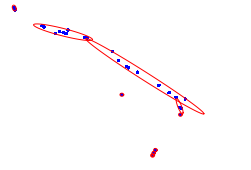
\includegraphics[width = 90mm]{images/gpsTrace.png}
			\caption[User's Location Trace]
			{The blue dots represent the user’s traces in a two-hour epoch over multiple days, and the red ellipses represent the clusters fitted. The major two directional clusters correspond to the user’s trajectory on a highway}
		\end{figure}		
		Once the user model is built and the profile completed, the algorithm can determine the likelihood of a random user of the phone not being the owner of the phone (the one whose user model was profiled). 
		
		As demonstrated by Shi et al., there are numerous ways contextual information can come in handy. In our case, we propose a default-context hybrid caching scheme for caching application components in memory, that operates by looking into the user's calendar for contextual information.  			
	
\chapter{Challenges in Collecting the Metrics}
	
	\section{Introduction}
		Now that we have laid the foundation for using contextual information to influence which processes Android caches in memory, we need to establish the metrics that need to be collected in order to measure the efficiency of the existing caching scheme and the proposed caching scheme. The following section addresses the metrics we need.
	
	\section{What are the desired metrics?}
		
		\subsection{Hits, Misses, Hit Ratio \& Latency}
			Alan Jay Smith defines Cache as a high speed buffer that holds items in current use [9]. In our context, Android holds application components (such as processes) as CBP (Cached Background Process)(s) in memory. As previously discussed, CBP(s) do not take up processor time, they are merely cached for quick application startup should the user request that particular application. A cache hit is a state in which data requested for processing by a component or application is found in the cache memory. It is a faster means of delivering data to the processor, as the cache already contains the requested data [10]. When applied to our scenario, a cache hit would represent a situation wherein the user requests (clicks) an application that currently resides in memory, either as an active process (including services) or as a CBP (Figure 3-1).  
			
			\begin{figure}[!ht]
				\centering
				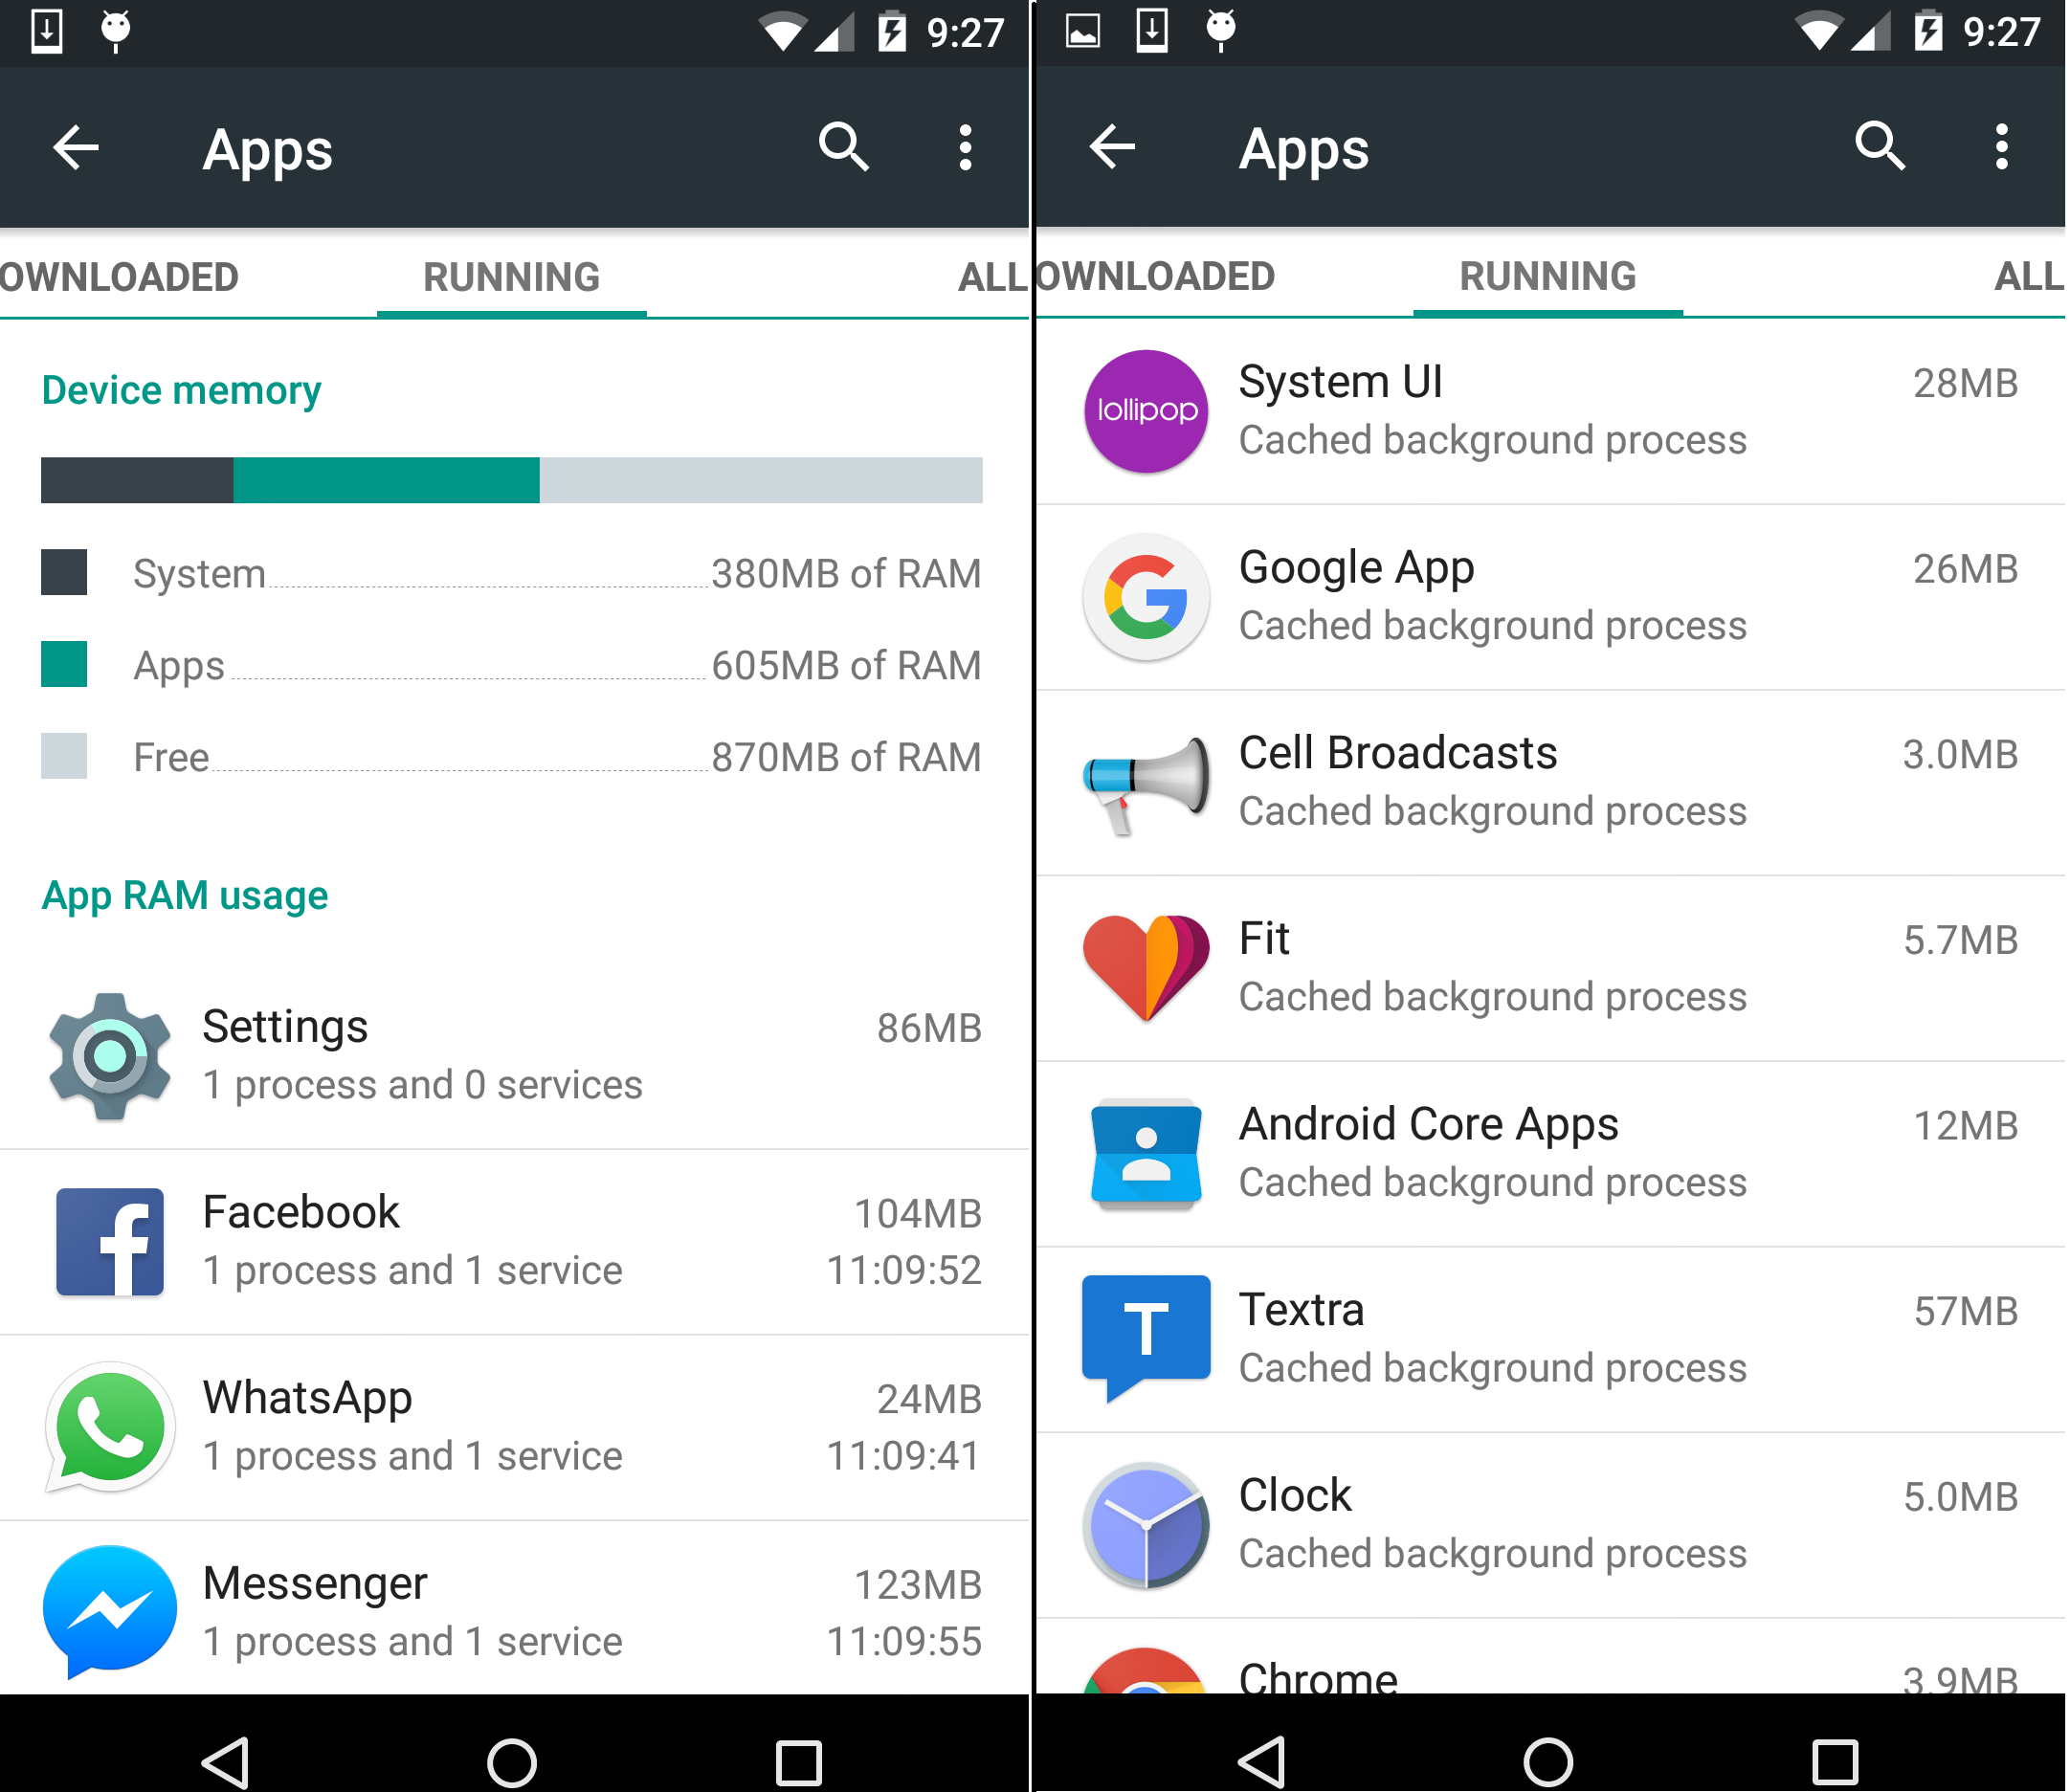
\includegraphics[width = 90mm]{images/runningApps.png}
				\caption[Running Applications and CBP(s) - Cache Hit]
				{Given this snapshot of the RAM, if the user clicks on say, the Messenger application (active process) or the Clock application (CBP), it would result in a Cache Hit}
			\end{figure}
			
			A cache miss is a state where the data requested for processing, by a component or application is not found in the cache memory [11]. When applied to our scenario, a cache miss would represent a situation wherein the user requests (clicks) an application that currently does not reside in memory, either as an active process (including services) or as a CBP (Figure 3-2).
			
			\begin{figure}[!ht]
				\centering
				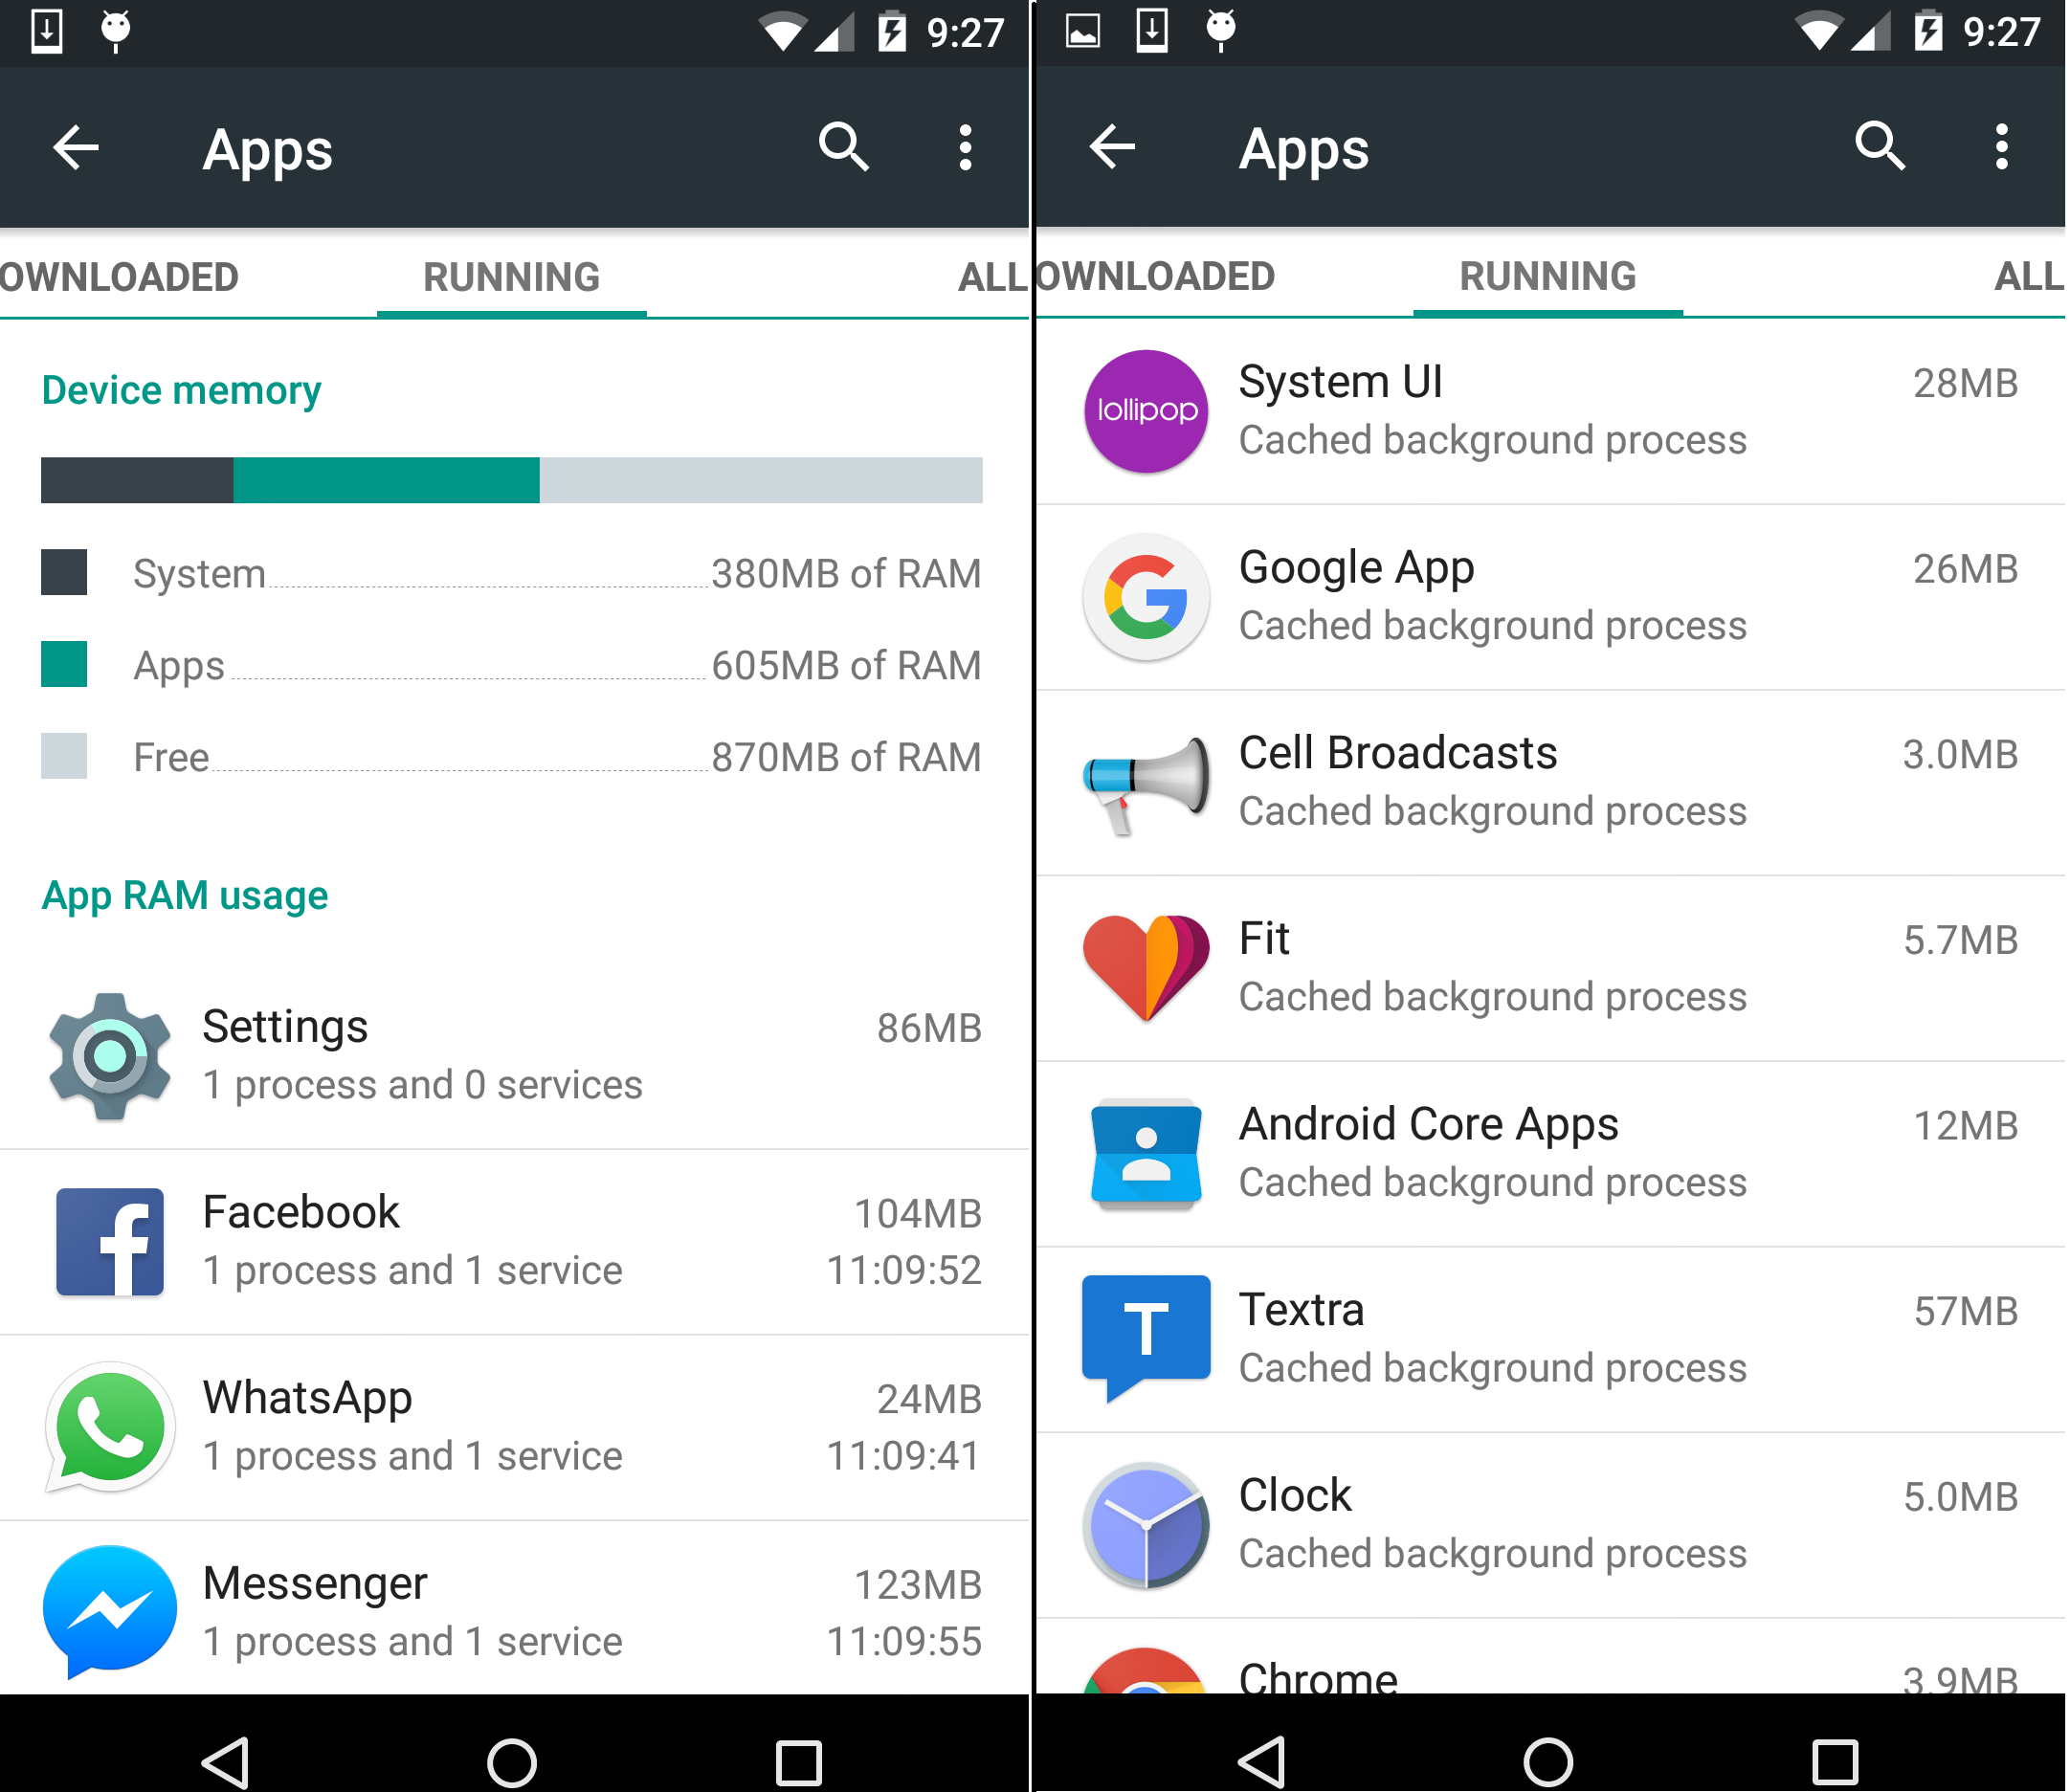
\includegraphics[width = 90mm]{images/runningApps.png}
				\caption[Running Applications and CBP(s) - Cache Miss]
				{Given this snapshot of the RAM, if the user clicks on say, the Google Drive application (process not in memory), it would result in a Cache Miss}
			\end{figure}		
			
			CHR (Cache Hit Ratio) is defined as the ratio of cache hits to the overall number of requests (total of cache hits and cache misses).
			
			\begin{eqnarray}
				Overall Number Of Requests = Cache Hits + Cache Misses \label{Total Requests} \\
				CHR = \frac{Cache Hits}{Overall Number Of Requests} \label{CHR} \\
				CHR'(In \%) = CHR * 100 
			\end{eqnarray}
			
			There are two primary figures of merit of a cache [9]:
			
			\begin{itemize}
				\item Latency
				\item CHR
			\end{itemize}
			
			The latency of a cache describes how long after requesting a desired item, the cache can return that item (in the case of a cache hit). In our scenario, processes are cached in RAM. Therefore, even if the number of processes cached in memory increases, there will hardly be any difference in the time it takes to fetch a requested item (application component) as they all reside in RAM which by definition supports random access. Latency is more of a factor in caches that are located further away from physical memory (such as L1 and L2 caches).
			
			The CHR of a cache describes how often a searched-for item is actually found in the cache. The higher the CHR, the better the cache is. When applied to our context, a high CHR results is more application components being fetched from memory, rather than disk which in turn results in quicker application startup times. This improvement in startup speed results in an enhanced user experience.   
		
		\subsection{Caching Schemes Under Consideration}
			Now that we have determined the fundamental metrics we need, let us analyze the various caching schemes under consideration.
			
			\subsubsection{Optimal Caching Scheme}
				The most efficient caching scheme would always have the requested item in cache. In our case, the ideal scheme would be one that ensures that every application the user requests, resides in memory. This optimal result is referred to as Belady's optimal algorithm [12] or the clairvoyant algorithm. Since it is generally impossible to predict the exact behavior of the user, this is not implementable in practice. The practical minimum can be calculated only after experimentation, and one can compare the effectiveness of the actually chosen caching scheme against Belady's as a benchmark.
			
			\subsubsection{Recency of Usage}
				This caching scheme primarily relies on recency of application usage and this is the default scheme Android currently uses. Android caches application components in memory as CBP(s) and associates each with a time-stamp. If the memory gets too full, it starts removing the least recently used CBP(s) first and depending on how direly low the memory is, it may not stop killing processes until even the active foreground application (the one user is interacting with) is removed [3], although this situation is extremely rare in practice and only results in the case of malfunctioning applications that leak memory. The Settings application can give the user clues about which CBP(s) were recently used. Clicking on an application that is currently not in memory results in that application being cached as a CBP near the top of the list. This suggests that the CBP(s) displayed by the Settings application are roughly sorted by their time-stamp from most recently used to least recently used (Figure 3-3). 
				
				\begin{figure}[!ht]
					\centering
					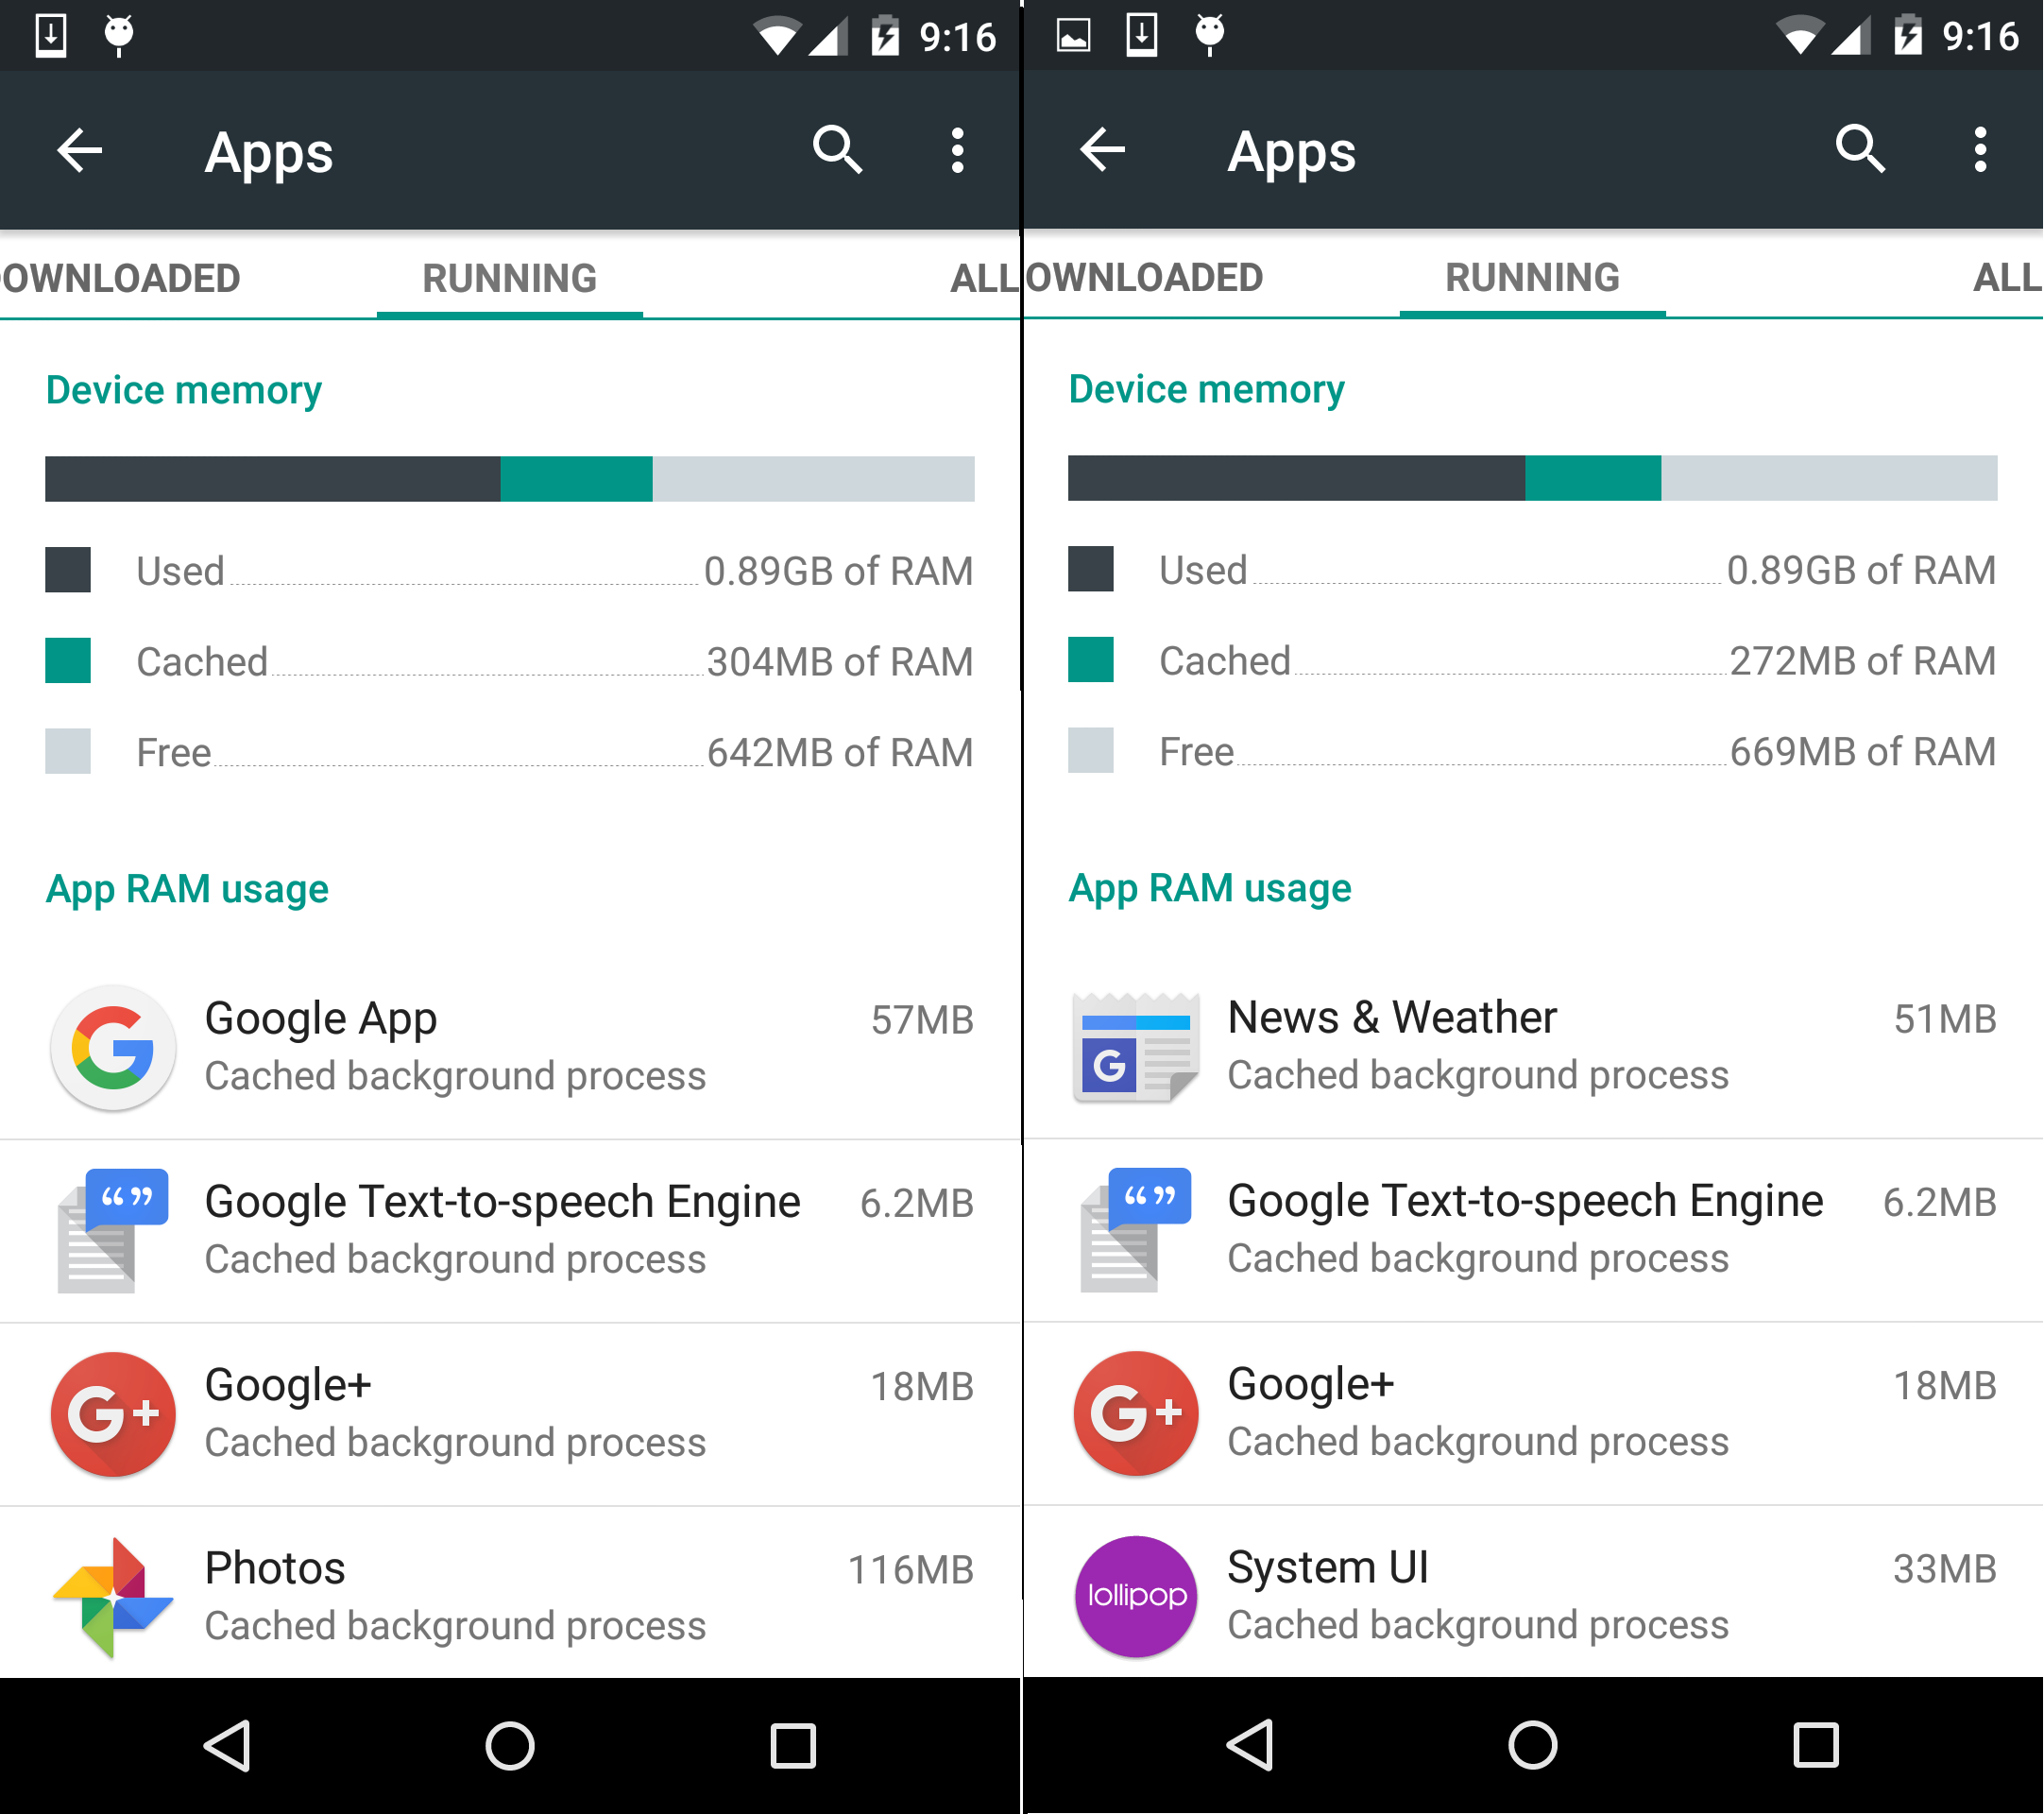
\includegraphics[width = 90mm]{images/beforeAndAfterNews.png}
					\caption[Before \& After News Application Launch]
					{The image to the left describes the snapshot of the CBP(s) as displayed to the end-user by the Settings application. The image to the right displays the snapshot of the CBP(s) after the end-user requests for the News and Weather application. Note that the News and Weather application will not be cached as a CBP until the user is done interacting with it as up until that point, it will reside in memory as an active process.}
				\end{figure}				
				
				It is worth noting that a perfect implementation of this caching scheme requires a time-stamp on each reference, and the OS needs to keep a list of items ordered by the time-stamp. This implementation may be deemed too expensive in certain cases especially if the frequency of memory references is high. The common practice is to approximate the behavior of this scheme [13].
			
			\subsubsection{Frequency of Usage}
				This caching scheme relies on the frequency of application usage as opposed to the recency of application usage. To elaborate, the most frequently used applications would be cached as CBP(s) in memory. This could be a really good alternative to the default recency-based scheme, given the tendency of most smartphone users to stick with the same set of popular applications and use them in rotation [15]. Under these circumstances, the frequency of a select few applications would be really high and would always be cached in memory as they are requested often. Frequency based caching scheme is sometimes combined with a recency-based caching scheme to form a frequency-recency hybrid [14].
				 
			\subsubsection{Random}
				Much like the name suggests this caching scheme would randomly select an application and cache it in memory as a CBP. This scheme does not require keeping any information about the access history. For its simplicity, it has been used in ARM processors [16]. When applied to our scenario, it does not seem like a viable option, mainly because there is not a benefit in randomly caching applications in memory.
				 
			\subsubsection{Default-Context Hybrid}
				So far we have analyzed the standard caching schemes that focus on caching items that were either accessed recently, frequently or in other ways that analyze past behavior. Our approach combines the applications that Android caches through a recency of usage scheme, with a separate context-analyzer module that reads the user's calendar and predicts which applications the user is likely to use. When the user requests an application, the combined set of applications (default applications based on recency and the list of predicted applications) is used as the base to compute whether a cache hit or a cache miss occurred. We will analyze in detail how each module functions but before that we need to examine two things:
				
				\begin{itemize}
					\item Whether Android can pro-actively cache application components in memory.
					\item Which applications will be removed from memory when it runs too low.
				\end{itemize}
								
				\paragraph{Pro-actively Adding CBP(s)}
					In order for the proposed Default-Context Hybrid (henceforth referred to as Hybrid) caching scheme to work, there must be provision for the Android OS to pro-actively cache application components in memory as CBP(s). Presuming that the context-analyzer module does its job and suggests a list of applications the user might use in the near future, there must a mechanism for Android to utilize that information and pro-actively cache these applications in RAM as CBP(s). This mechanism can be verified at the user level through a small experiment. As previously mentioned, the Settings application provides a visual interface for the list of active processes and services running in memory and the CBP(s) that reside in memory at any moment in time. As part of the experiment, each and every CBP was forcefully removed from the cache (there is provision to do this at the user level (Figure 3-4)). 
						
					\begin{figure}[!ht]
						\centering
						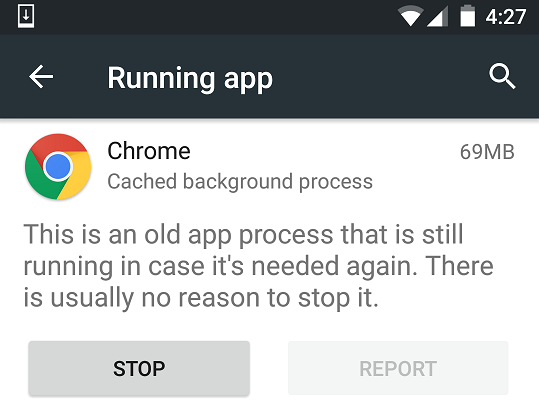
\includegraphics[width = 90mm]{images/removeCBP3.png}
						\caption[Remove CBP]
						{Pressing the {\em STOP} button removes the CBP from memory}
					\end{figure}					
					
					Once each CBP was removed, the phone was untouched for three minutes. After three minutes, when the Settings application was launched to look at the list of CBP(s), it was not empty. Instead, there were several CBP(s), some of which were previously removed and some of which were not in the list to begin with (Figure 3-5). 
					
					\begin{figure}[!ht]
						\centering
						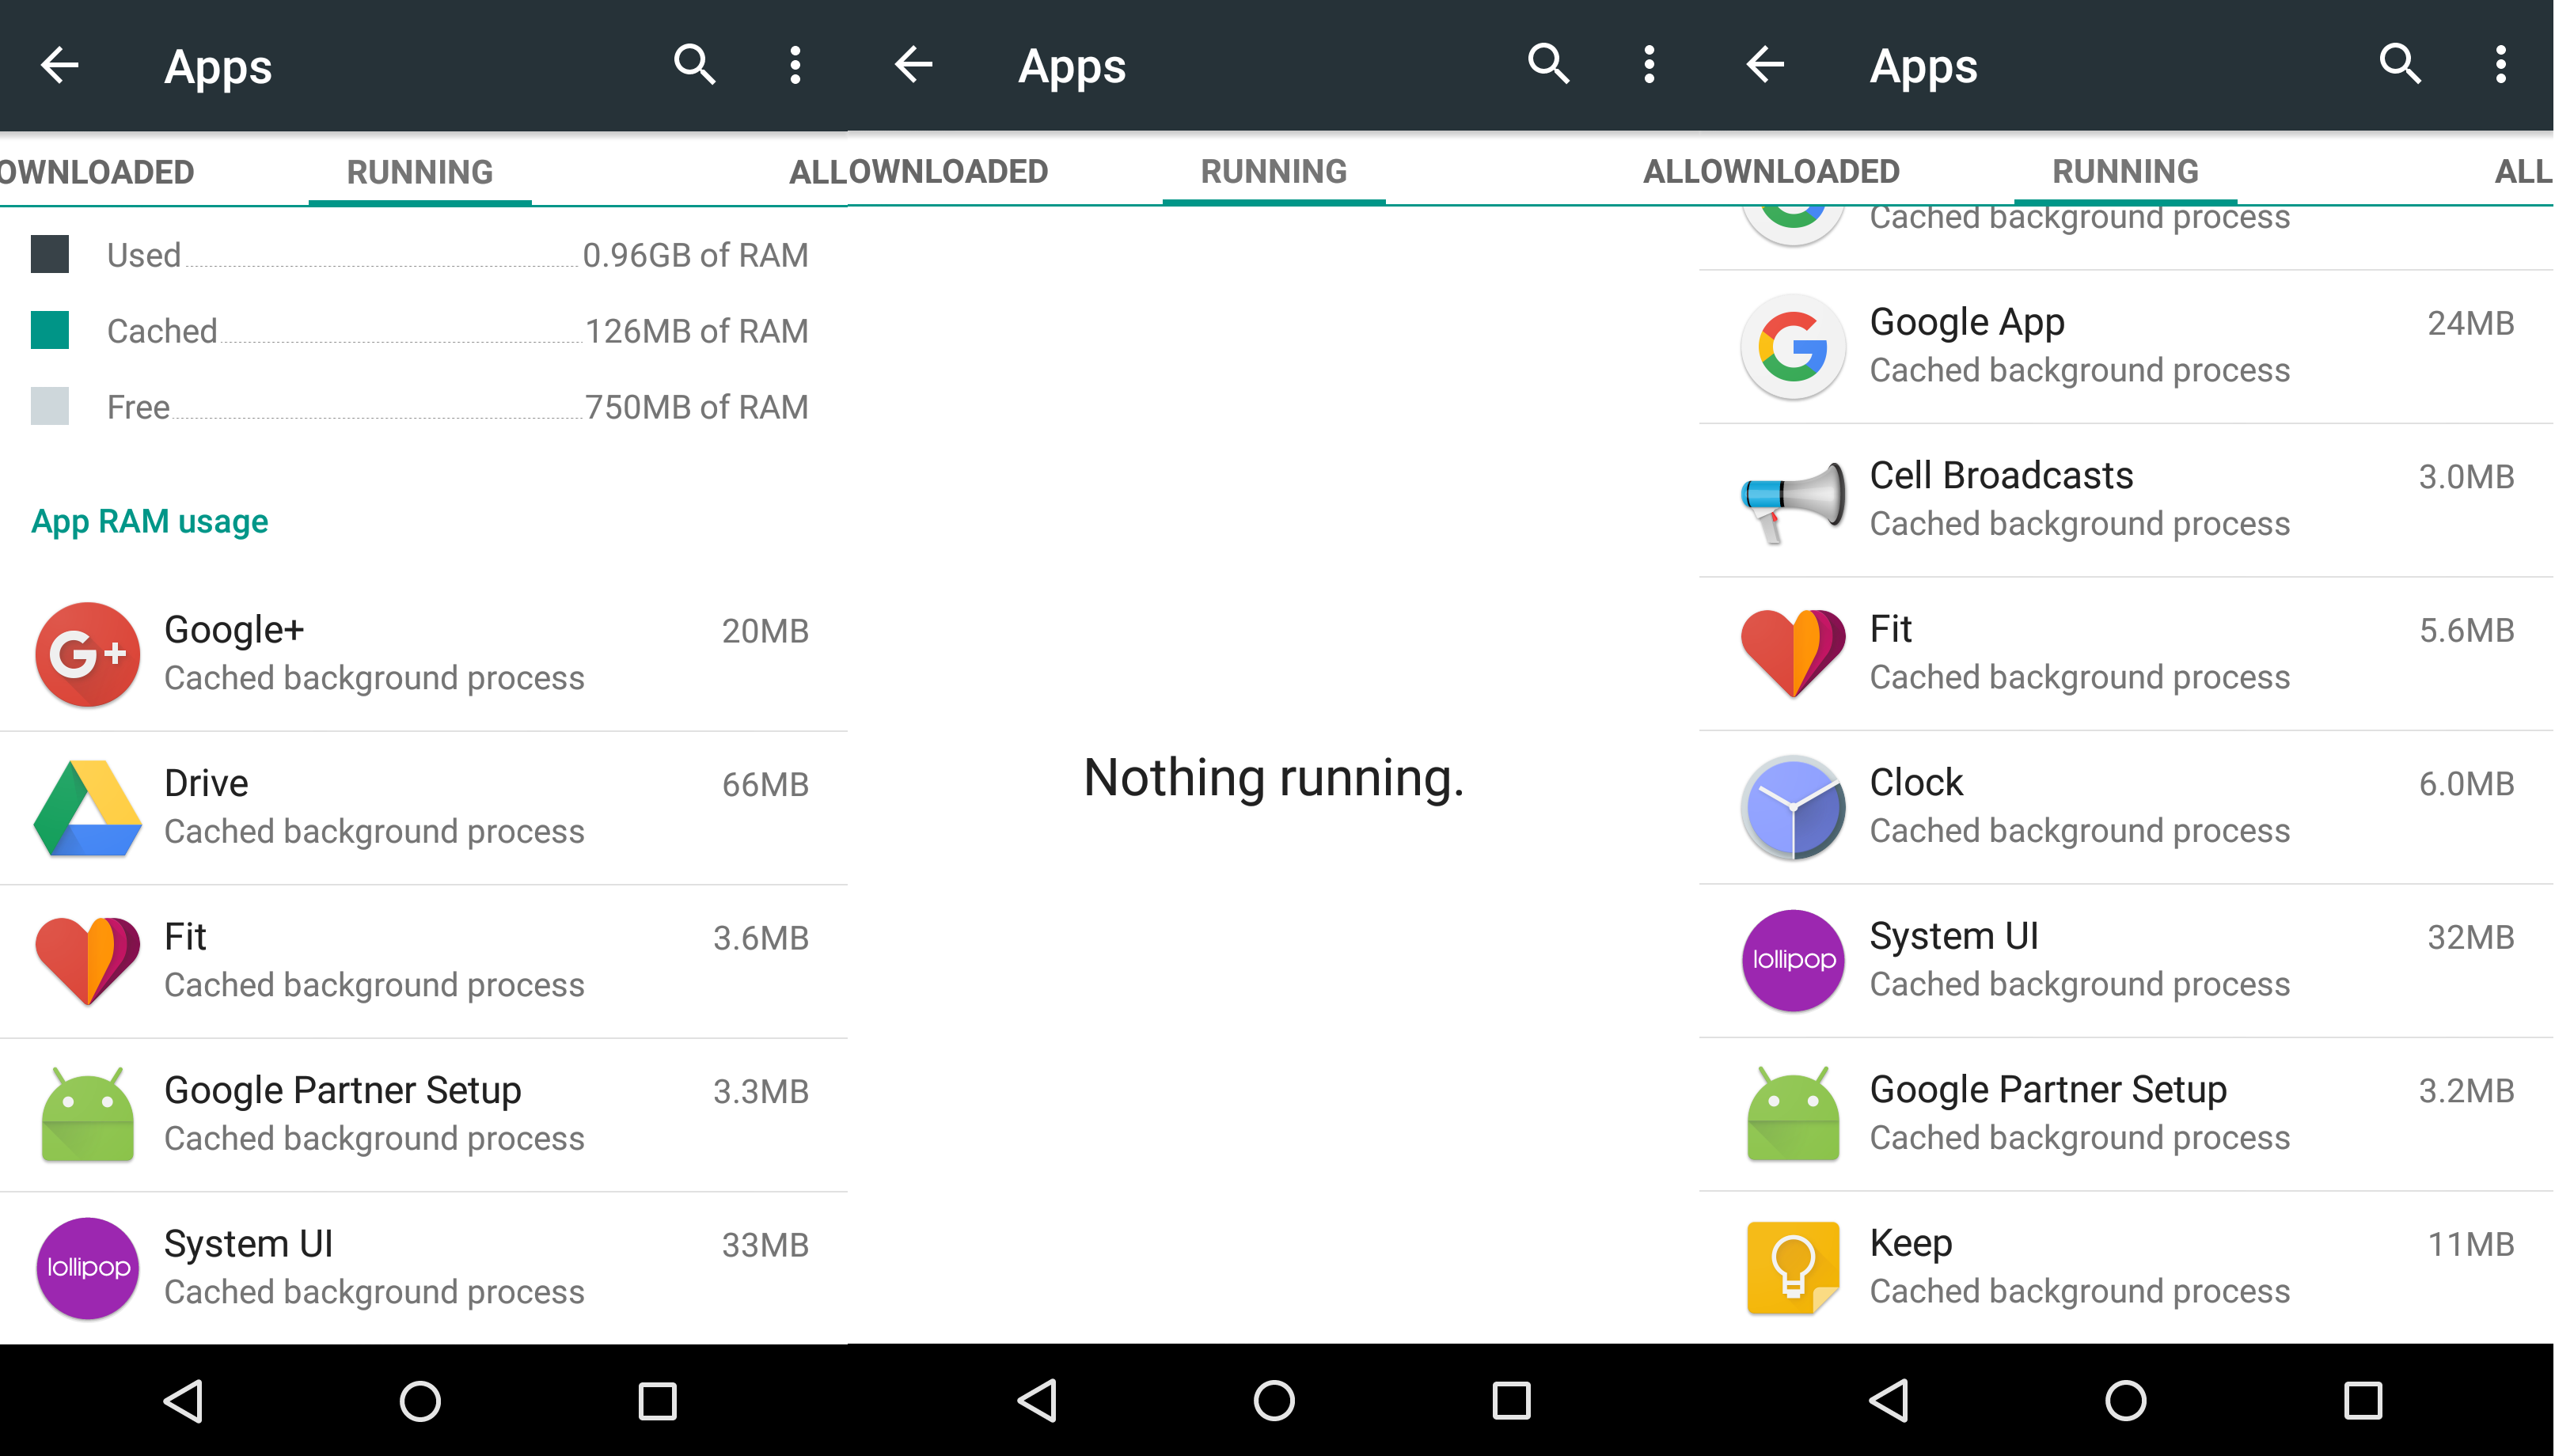
\includegraphics[width = 130mm]{images/stage123.png}
						\caption[CBP(s) before and after manual removal]
						{The leftmost image shows the snapshot of the CBP(s) before forceful deletion. After each and every CBP was removed manually, the screen displayed is shown in the middle image. The image farthest to the right shows the repopulated list of CBP(s), 3 minutes after the middle image was taken. This demonstrates Android's ability to utilize free RAM space and pro-actively cache CBP(s)}
					\end{figure}					
					
					This indicates that Android pro-actively caches applications that were not in memory to begin with, as CBP(s). This is also the reason why task killer applications fell out of favor [17]. This demonstrates that not only does Android provide a mechanism to pro-actively cache applications in memory, it already does so. The applications suggested by the Hybrid scheme can be introduced into the memory as CBP(s) in the same way. This is discussed in Chapter 8.

				\paragraph{Prioritizing Applications in Hybrid Scheme}	
					The Hybrid scheme would involve storing as CBP(s), both default application components cached by Android's recency-based scheme and the application components of the list of applications obtained from analyzing the user's calendar. So the question now becomes, who gets kicked out when memory is running low? Since the applications inferred from user's contextual information do not have a recency associated with them, the overall list of CBP(s) cannot be prioritized based on recency of usage. A simple solution is to prioritize the CBP(s) obtained from the list of suggested applications over the default ones i.e. all the default CBP(s) are removed from memory before the CBP(s) cached as a result of context inference. Alternatively, the CBP(s) with the least memory footprint can be prioritized i.e. the most memory-heavy CBP(s) are removed first. While this approach releases memory quickly, it does not take into account the likelihood of application usage in the immediate future.
					
		\subsection{Supplementary Data}
			We have talked about the fundamental metrics involved in measuring the efficiency of any caching scheme, namely cache hits, cache misses and CHR. We explored potential candidates for serving as the caching scheme in managing the list of CBP(s) cached in memory. There are other subtle measurements that are not as significant as the fundamental metrics but are important nonetheless as they shed light on certain attributes of the experiment. They are listed below:
			
			\begin{itemize}
				\item Number of Installed Applications
				\item Number of Unique Applications Requested (Clicked)
				\item Number of Calendar Entries During the Course of the Experiment
				\item Phone Model
				\item Android OS Version
			\end{itemize} 
			
			These are elaborated upon in Chapter 5 under the demographic data section.   
			
	\section{Challenges}
		Now that we have established what the desired metrics are, let us examine some of the challenges in collecting them.  
		
		\subsection{Deciding Between System vs User Level Approach}
			Firstly, we need to determine whether to approach the problem from a user level perspective or not. Attempting to solve the problem i.e. collecting the aforementioned metrics at the user level would involve building Android applications to gather relevant data. On the other hand, approaching the problem from a system level would involve altering the source code of the Android OS (facilitated by AOSP) and recompiling it to build our own custom distribution, much like the CyanogenMod community [18]. It is easier to solve the problem (if possible) at the user level for two reasons:
			
			\begin{itemize}
				\item The complexity involved in altering OS source code is significantly higher compared to writing Android applications.
				\item It would be significantly harder to convince potential research volunteers to reboot their smartphones with a custom distribution of the Android OS as opposed to asking them to install an Android application.
			\end{itemize}
			
			Given that it is beneficial to gather relevant data at the user level, we need to identify the complexities involved and determine whether they are solvable at the user level. In order to effectively determine which caching scheme is ideal for caching CBP(s) in memory, we need to identify whether the following problems can be approached from a user level perspective:
			
			\begin{itemize}
				\item Getting the list of processes currently in memory \checkmark
				\item Knowing when a new process is launched by the user \checkmark
				\item Reading the User's Calendar \checkmark
			\end{itemize} 
			
			We will inspect in detail, why and how we need to solve these problems (and others) in the next section. The  '\checkmark' indicates that they are indeed solvable at the user level and do not require system level changes.
			
		\subsection{Getting Processes in Memory}
			Let us first address why it is necessary to get the list of processes that reside in memory. In our scenario, we are trying to determine the most efficient caching scheme among the following:
			
			\begin{itemize}
				\item Default Recency based Scheme
				\item Pure Context Scheme (Applications will be cached solely based on context inference)
				\item Default-Context Hybrid (or simply Hybrid)
			\end{itemize}
			
			In order to determine which scheme is most efficient, we need the ability to measure CHR data and by extension if and when a cache hit or miss occurs. We can only determine if a cache hit occurred if we had access to the list of processes in the cache i.e. the active processes and the CBP(s) in memory. The {\em ActivityManager} class in Android provides two relevant helper methods [19]:
			
			\begin{itemize}
				\item {\em getRunningTasks()}
				\item {\em getRunningAppProcesses()}
			\end{itemize} 
			
			Unfortunately, as of Android 5.0, it has become increasingly difficult to get a list of applications running in memory. {\em getRunningTasks()} has been deprecated and {\em getRunningAppProcesses()} has been killed (It only returns the requesting application rather than all applications running in memory). An alternate solution is to use the {\em UsageStatsManager} class [20]. However, it requires special permission from the user in the Settings application and some OEM (Original Equipment Manufacturers)(s) have removed this setting explicitly, rendering this solution unreliable. The best solution involves using the ADB (Android Debug Bridge) shell to retrieve the desired information which can then be parsed into a suitable list of processes residing in memory. ADB is a versatile command line tool that enables communication with an APMD. It is a client-server program that includes three components [21]:
			
			\begin{itemize}
				\item A client, which runs on the APMD. The client can be invoked from a shell by issuing an ADB command.
				\item A server, which runs as a background process on the APMD. The server manages communication between the client and the ADB daemon running on the APMD.
				\item A daemon, which runs as a background process on the APMD.
			\end{itemize}
			
			The ADB provides a Unix shell that can be used to run a variety of commands on the APMD. The command binaries are stored in the APMD's file system at {\em /system/bin/} [22]. We obtain the list of processes residing in memory by running the {\em toolbox} command [26] in the shell. The Android {\em toolbox} command encapsulates the functionality of many common Linux commands (and some special Android commands) into a single binary [23]. Of these, we are most interested in the {\em toolbox} and {\em ps} commands as they provide a direct window into the processes residing in memory. 
			
%			We use the following parameters with the {\em toolbox ps} command to get the desired process data:
%			
%			\begin{itemize}
%				\item '-P': It shows the scheduling policy.
%				\item '-p': It displays the priorities and niceness level.
%				\item '-x': It shows system time in seconds
%				\item '-c': It displays the CPU
%			\end{itemize}
%			
			With the help of {\em libsuperuser} library which provides a convenient framework to run shell commands [24] and the {\em AndroidProcess} library which provides a framework to parse the process-related shell outputs [25], the following algorithm (Algorithm 1) was written to obtain a list of processes residing in memory (active processes and CBP(s)). It is worth noting that this list corresponds to the list of processes displayed by the Settings application (Figure 3-1) as part of the running applications and CBP screens, and that the Settings application has system privileges that third party Android applications do not.\\ 
			
			\begin{algorithm}[H]
				\SetAlgoLined
				\KwResult{LIST Process}
				
				INITIALIZE LIST Process - processes\\
				LIST String - stdout --- Shell.SH.run("toolbox ps -p -P -x -c")\\
				Integer myPid 		 --- android.os.Process.myPid()
				
				\For{String line : stdout}
				{
					INITIALIZE Process - process\\
					\eIf{process matches APP-ID-PATTERN}
					{
						\eIf{(process.ppid EQUAL TO myPid)\\ OR (process.name EQUAL TO "toolbox")}
						{
							CONTINUE
						}
						{
							ADD TO processes - process
						}
					}
					{
						CONTINUE
					}
				}
				
				RETURN processes;\\
			
			\caption[Algorithm to get list of processes in RAM]{In the above algorithm, {\em Process} is a custom data structure that parses the output format of the {\em toolbox ps} command. Its class structure is discussed in Chapter 4. The {\em APP-ID-PATTERN} is a regular expression that maps to application ID patterns for the Android OS in versions 5.0 and above. Each process is added to a result list that is returned by the algorithm. Note that the requesting application represented by {\em myPid} (discussed in 4.4) and {\em toolbox} related processes represented by process names that match {\em toolbox}, are not added to the result.}
			\end{algorithm}			
			
		\subsection{Obtaining the Foreground Application}
			In order to update the CHR metric, we need the ability to detect new cache hits and cache misses. A new cache hit/miss occurs when there are new application requests i.e. changes in the foreground application. Before we analyze how to detect change in the foreground application, we first need a way to obtain the current foreground application. Had we approached this problem at the system level, we could have made use of system level privileges such as listening to a new screen-touch by the user and detecting which application was  launched but this is not possible from a third party user-level application. Fortunately, there is a workaround to detecting the foreground application at the user level. We obtain every process currently running in memory and through a process of elimination, obtain the process associated with the foreground application. To elaborate, the foreground application has certain unique properties in its process name, UID (Unique Identifier) and other fields, that can be exploited to eliminate processes that are not associated with the current foreground application. The following   algorithm (Algorithm 2) illustrates this process.
			
			\begin{algorithm}[H]
				\SetAlgoLined
				\KwResult{Foreground Application}
				
				INITIALIZE LIST {\em files} --- LIST {\em /proc} File\\
				\For{File file : files}
				{
					\If{file IS A DIRECTORY}{CONTINUE}
					
					{\em pid --- file.getName()}\\
					{\em cgroup} --- FILE READ ({\em /proc/\%d/cgroup})\\
					{\em cpuSubSystem, cpuAccountSubSystem --- cgroup}\\
					
					\If{cpuAccountSubSystem ENDS WITH pid OR cpuSubSystem ENDS WITH bg\_non\_interactive}{CONTINUE}
					
					{\em cmdline} --- FILE READ ({\em /proc/\%d/cmdline})\\
					{\em uid} --- PARSE FROM {\em cpuAccountSubSystem}\\
					
					\If{cmdline CONTAINS com.android.systemui OR uid BETWEEN 1000 AND 1038}{CONTINUE}
					
					{\em oomAdj} --- FILE READ ({\em /proc/\%d/oom\_score\_adj})\\
					{\em oomScore} --- FILE READ ({\em /proc/\%d/oom\_score})\\
					
					\If{LOWEST oomScore AND oomAdj EQUAL TO 0}{RETURN cmdline}
				}
				
				\caption[Algorithm to get current foreground application]{This algorithm obtains the current foreground process i.e. the process associated with the application that the user is interacting with.}
			\end{algorithm}
			
			Firstly, all files with path {\em /proc} are obtained and each iterated over, to find the foreground application. We eliminate file directories as these are of no concern to us. If the CPU account sub-system ends with {\em pid}, it is not an application process and is thus eliminated. Similarly, if the CPU sub-system ends with {\em bg\_non\_interactive}, it is a background process and is eliminated as well. The application stored in {\em cmdline} is a potential candidate for the foreground application and is the right choice as long as it clears four more hurdles:
			
			\begin{itemize}
				\item {\em cmdline} does not contain {\em com.android.systemui}
				\item {\em uid} does not lie between 1000 and 1038
				\item {\em oomAdj} i.e. the OOM (Out Of Memory) adjustment level [27] equals 0
				\item {\em oomScore} is the lowest among all iterated values
			\end{itemize}
			
			If {\em cmdline} contains {\em com.android.systemui} or if {\em uid} lies between 1000 and 1038, it is a system application and is thus eliminated from consideration. The crucial attribute of the foreground application is that it has the lowest OOM score of all applications. When the Android OS is running too low on memory, it is the job of the Linux OOM killer [28] to sacrifice one or more processes in order to free up memory for the system when all else fails. A low OOM score indicates that the process is less likely to be killed and that it is lower on the OOM killer's radar. The process with the lowest OOM score is the foreground process as it is of paramount importance not to remove the process the end-user is interacting with, unless as a last resort. This unique property of the foreground process enables us to distinguish it from the rest of the pool. 
			
		\subsection{Updating the Statistics}
			 So far, we have established ways to collect the list of processes in memory and the foreground application. The next step is to figure out a way to update the metrics as and when the user requests new applications. The rate at which the end-user toggles between applications varies from person to person. It also depends on the level of usage. For instance, there are times when the end-user is actively using their APMD and others when the APMD is idle or switched off. Therefore it is hard to predict when there could be a potential change in the foreground application. There is no inherent mechanism for user-level applications to detect third party application launches (That privilege is reserved for system level processes). Therefore, our solution comprises of starting a service [2] that retrieves the current foreground process (Algorithm 2) and the current list of processes residing in memory (Algorithm 1) every second. If there is a change detected in the foreground process (compared to the last second), then the cache metrics are updated. The time interval of one second is chosen as it is deemed to be reasonably accommodative of the average time it takes an end-user to switch from one application to another. This is further discussed in Chapter 8. The design of the service and the corresponding application is discussed in Chapter 4. The following algorithm (Algorithm 3) illustrates the process of updating the cache metrics.\\     
			 
		 	\begin{algorithm}[H]
		 		\SetAlgoLined
		 		\KwResult{Update Cache Metrics}
		 				 		
		 		\For{EACH SECOND}
		 		{	
		 			{\em newForegroundApp --- getNewForegroundApp()}\\
		 			{\em currentListOfProc --- getListOfProcesses()}\\	 			
		 			\If{newForegroundApp EQUALS oldForegroundApp}{CONTINUE}
		 			\eIf{oldListOfProc CONTAINS newForegroundApp}{cacheHit++}{cacheMiss++}
		 			{\em updateMetrics()}\\
		 			{\em oldListOfProc --- newListOfProc}\\
		 			{\em oldForegroundApp --- newForegroundApp}		 			
		 		}
		 		
		 		\caption[Algorithm to update cache metrics]{This algorithm retrieves the foreground application and checks if it has changed since the last second. If it has, it verifies whether it was a cache hit or a cache miss and updates the cache metrics. Finally, it updates the old foreground application and the previous list of processes to the current one so that the next iteration uses these values as the base.}
		 	\end{algorithm}

		\subsection{Backing Up the Data}
			Previously, we discussed the mechanism by which the background service updates the cache metrics. The other aspect of this issue is storing this data. Before we inspect how to store the data, let us discuss the necessity for such a provision. Our background service is designed to run throughout the duration of the experiment and retrieve the foreground application and the list of processes in memory every second. This results in it is OOM score increasing i.e. it is likelihood of getting killed by the Linux OOM killer [28] which would result in a loss of data. It is worth noting that the OOM killer selects the {\em best} process to kill which is decided by the combination of how long a process has been running and how much memory would be released if the process is killed. Even though our process scores poorly on the time duration aspect, it takes up relatively low memory compared to some of the other common background processes (Figure 3-6).

			\begin{figure}[h]
				\centering
				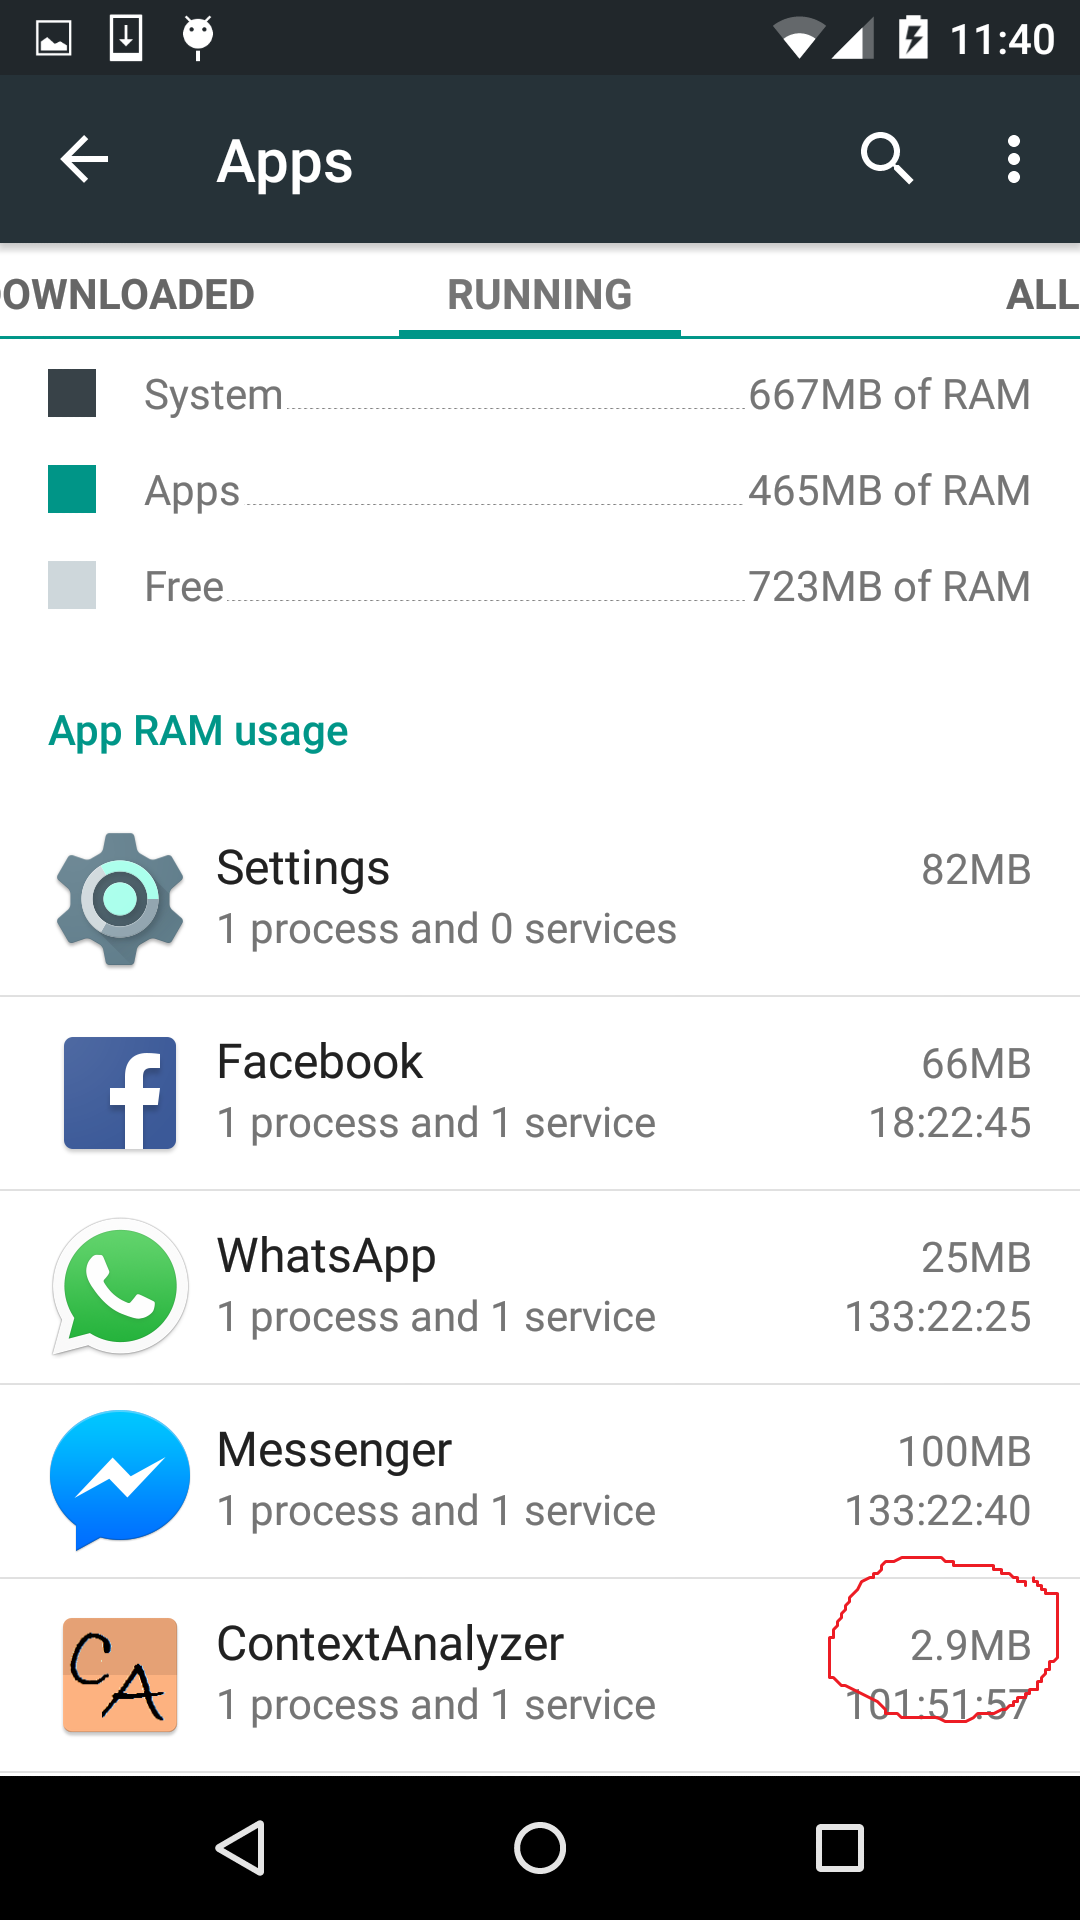
\includegraphics[width = 70mm]{images/lowMemory.png}
				\caption[Memory Occupied by the Background Service]{{\em ContextAnalyzer} is our custom Android application that reads the user's calendar and collects cache metrics. The service mentioned in the diagram is the background service that updates the metrics every second. We will discuss the design of this application in Chapter 4. it is worth noting that the memory footprint of the application is quite low. This is not to suggest that it will not get killed by the OOM killer (as its longevity is still a factor), which is why we are backing the data up.}
			\end{figure} 

			Android provides several options for saving persistent application data. There are five ways to accomplish this task [29]:
			
			\begin{itemize}
				\item Shared Preferences - It is used in cases where primitive data needs to be stored in Key Value pairs.
				\item Internal Storage - It is used to store private data on device memory.
				\item External Storage - It is used to store public data on shared external storage
				\item SQLite Databases - They are used to store structured data in a relational database.
				\item Network Connection - It is used to store data over the Internet.
			\end{itemize}
			
			For our scenario, Internal Storage is the best fit as it keeps the data private to the application and since the data is quite primitive (cache hits and misses), we do not need SQLite databases or network connections. The data is written to a file every minute. That way, we do not have to constantly perform I/O operations from the service and in the worst case scenario, fifty nine seconds of Cache data would be lost which is relatively a small amount of time. Algorithm 3 can be tweaked to incorporate the file write operation (Algorithm 4).
			
			\begin{algorithm}[H]
				\SetAlgoLined
				\KwResult{Update Cache Metrics AND Write to File}
				
				\For{EACH SECOND}
				{	
					...\\
					...\\
					{\em updateMetrics()}\\
					\If{END OF MINUTE}{ writeMetricsToFile()}
					...\\
					...\\	
				}
				
				\caption[Modified Update Metrics Algorithm]{In addition to updating the metrics every second, it also writes the data to internal storage every minute. Any time the application is closed and launched again the metrics are initialized with the values in file.}
			\end{algorithm}
			
		\subsection{Reading the User's Calendar}
			To compute the CHR of the Hybrid scheme, we need the ability to obtain the list of events from the user's calendar and the ability to parse that information to come up with a list of suggested applications. We will discuss the parsing aspect in the next segment and focus on finding a way to read the user's calendar. The solution to this problem is quite simple, Google provides a public API [30] to obtain access to the user's calendar information, including the list of events. We query the calendar every four hours (for events occurring in that four hour period) and feed the data (events list) into a module that parses the information and produces a suggested list of applications (Algorithm 5). 
			
			\begin{algorithm}[H]
				\SetAlgoLined
				\KwResult{Update Cache Metrics, Write to File AND Update List of Suggested Applications}
				
				\For{EACH SECOND}
				{	
					...\\
					...\\
					{\em updateMetrics()}\\
					\If{END OF MINUTE}{ writeMetricsToFile()}
					\If{END OF 4 HOURS}{updateListOfSuggestedApplications()}
					...\\
					...\\	
				}
				
				\caption[Update Suggested Applications List]{In addition to updating the metrics every second and writing them to file every minute, it also updates the list of applications suggested by the Calendar Parser (discussed in next segment)}
			\end{algorithm}
			
			The following algorithm (Algorithm 6) illustrates our implementation of the module that queries the user's calendar.
			
			\begin{algorithm}[H]
				\SetAlgoLined
				\KwResult{Get List of Events from Calendar}
				INITIALIZE List {\em result}\\
				List {\em allEvents} ---  QUERY {\em content://com.android.calendar/events}\\
				\For{EACH event IN allEvents}
				{	
					\If{event.startTime() IS WITHIN 4 hours FROM NOW}{result.add(event)}
				}
				RETURN result
				\caption[Algorithm to read user's calendar]{This algorithm obtains all events in the user's calendar that start within 4 hours from the time of the algorithm invocation.}
			\end{algorithm}
						
		\subsection{Parsing the Calendar Information}
			We have examined the mechanism behind reading the user's calendar, thereby solving one half of the puzzle. The other half is utilizing this information to compute the Hybrid scheme's metrics. In order to achieve that, we need to build a module that parses the list of events obtained from reading the calendar and suggests a list of applications. Every event in the user's calendar is split into individual keywords and a predetermined mapping between keywords and applications builds this list. The keyword-application mapping is determined by a two factors:
			
			\begin{itemize}
				
				\item There is a default application [42] that directly maps to the keyword.
					
					\begin{itemize}
						\item For instance the keyword {\em mail} is mapped to the {\em GMail} application, which is the default e-mail application in APMD(s).
						\item Similarly the keyword {\em call} is mapped to the {\em Google Dialer} application, which is the default application to make and receive calls.
					\end{itemize}
				
				\item Additionally, when the Google Play Store [32] is searched with the keyword, the top result is mapped to it.
					
					\begin{itemize}
						\item  For instance, when the Play Store was searched with the keyword {\em skype}, Skype application was the top result. Once it is verified that Skype is part of the installed applications [33], it is added to the list of suggested applications.
					\end{itemize}
					
			\end{itemize}

			Finally, if there are no events in the user's calendar for the four hour period, then the list of suggested applications is populated with a maximum of ten default applications. These default applications are derived from the ten most popular Android applications in USA (United States of America) [31]. Out of these ten applications, every application that the user has installed in their APMD will be added to the default list (resulting in a maximum of ten default applications).

\chapter{Experiment Setup and Application Design}
	
	\section{Introduction}
		In the previous chapter, we examined the metrics we needed to analyze the best caching scheme for caching application components in memory as CBP(s). We looked into some of the common caching schemes and analyzed some of the challenges in collecting the metrics needed to determine if contextual information can help better the CHR of the Hybrid approach. To analyze the efficiencies of the default recency-based approach and the Hybrid approaches, an Android application namely {\em ContextAnalyzer} was developed to collect the desired cache metrics. It was installed in the APMD(s) of research volunteers. We will dissect {\em ContextAnalyzer}'s design in Section 4.4.  
		
	\section{Eligibility for Volunteers}
		The following criteria had to be met to qualify as a research volunteer:
		
		\begin{itemize}
			\item The volunteer must own an APMD with Android OS version greater than 5.0 (Lollipop and above).
			\item The volunteer must be willing to install a third party application on their APMD.
		\end{itemize}
		
		The algorithm that obtains the list of processes currently residing in memory (Section 3.3.2) and the algorithm that retrieves the current foreground application (Section 3.3.3) do not apply to Android OS versions below 5.0, hence the necessity for APMD(s) with OS versions that are Lollipop and above.
		
		\subsection{Addressing Privacy Concerns}
			Since the research volunteers had to install a third party application ({\em ContextAnalyzer}), it was crucial to address any privacy concerns that arose. In order to gain the trust of the volunteers, we adopted a policy of full transparency and took the following measures:
			
			\begin{itemize}
				\item We fully explained to each volunteer, the nature of the data we were collecting i.e. cache metrics.
				\item We open sourced the Android application [35] in case the volunteers wanted to verify that there were no nefarious activities going on in the background.
				\item We did not automatically store the cache metrics in a server. Instead, we asked the volunteers to send us the data in order to convey the message that we were not collecting any private data that the volunteers were not aware of.
			\end{itemize}
			
			Although the aforementioned points address the privacy issues, we realize that divulging the nature of the experiment has the potential to bias the volunteers in their APMD usage. We explore this aspect in detail in Chapter 8. 
	
	\section{Process and Duration of Experiment}
		A total of twenty volunteers signed up and installed the application. Each volunteer had the application running for a minimum of 7 days and a maximum of 12 days. A 7 day minimum was enforced to ensure that the monitoring period included both weekdays and weekends. This accounted for any difference in usage patterns among the volunteers during the weekends. The link to the APK (Android Package) file was posted online [40] and each volunteer downloaded and installed the application as a third-party application. In this context, the term third-party refers to the fact that the Android application was not downloaded from the Google Play store. The volunteers were instructed not to manually stop the application for the duration of the experiment [36].
		 		 
	\section{Context Analyzer Design}
		{\em ContextAnalyzer} computes the metrics for both the default scheme and the Hybrid scheme. In order to  accomplish this, {\em ContextAnalyzer} reads the user's calendar (Section 3.3.6) and produces a list of applications that the user is likely to use. For the sake of simplicity, let us refer to this list as the calendar list. It also reads the list of processes residing in memory (Section 3.3.2). Let us refer to this list as the memory list. Given this information, every application that the user requests falls in one of four categories:
		
		\begin{itemize}
			\item The application is present in neither list.
			\item The application is present in memory list but not the calendar list.
			\item The application is present in calendar list but not the memory list.
			\item The application is present in both lists. 
		\end{itemize}  
		
		If the application is present in neither list, it results in an overall cache miss. To elaborate, an overall cache miss implies that neither the list of processes in memory (cached by the default recency-based caching scheme) nor the list of applications predicted by reading the calendar, contained the requested application. If the application was present only in memory list, it results in an overall cache hit and a suggested cache miss i.e. the Hybrid scheme would have still had a hit but it was not present in the list of applications suggested by the calendar list. If the application was present only in the calendar list, it results in an overall cache hit and a suggested-exclusive cache hit, implying that the hit is solely a result of the calendar list's suggestion. This metric is important as it reveals the significance of the list of applications suggested exclusively by the calendar list. Finally, if the application was present in both lists, it results in an overall cache hit and suggested non-exclusive cache hit, implying that the hit would have occurred regardless of whether the application was present in the calendar list or not. The following snapshot (Figure 4-1) illustrates {\em ContextAnalyzer}'s UI (User Interface).  
		
		\begin{figure}[h]
			\centering
			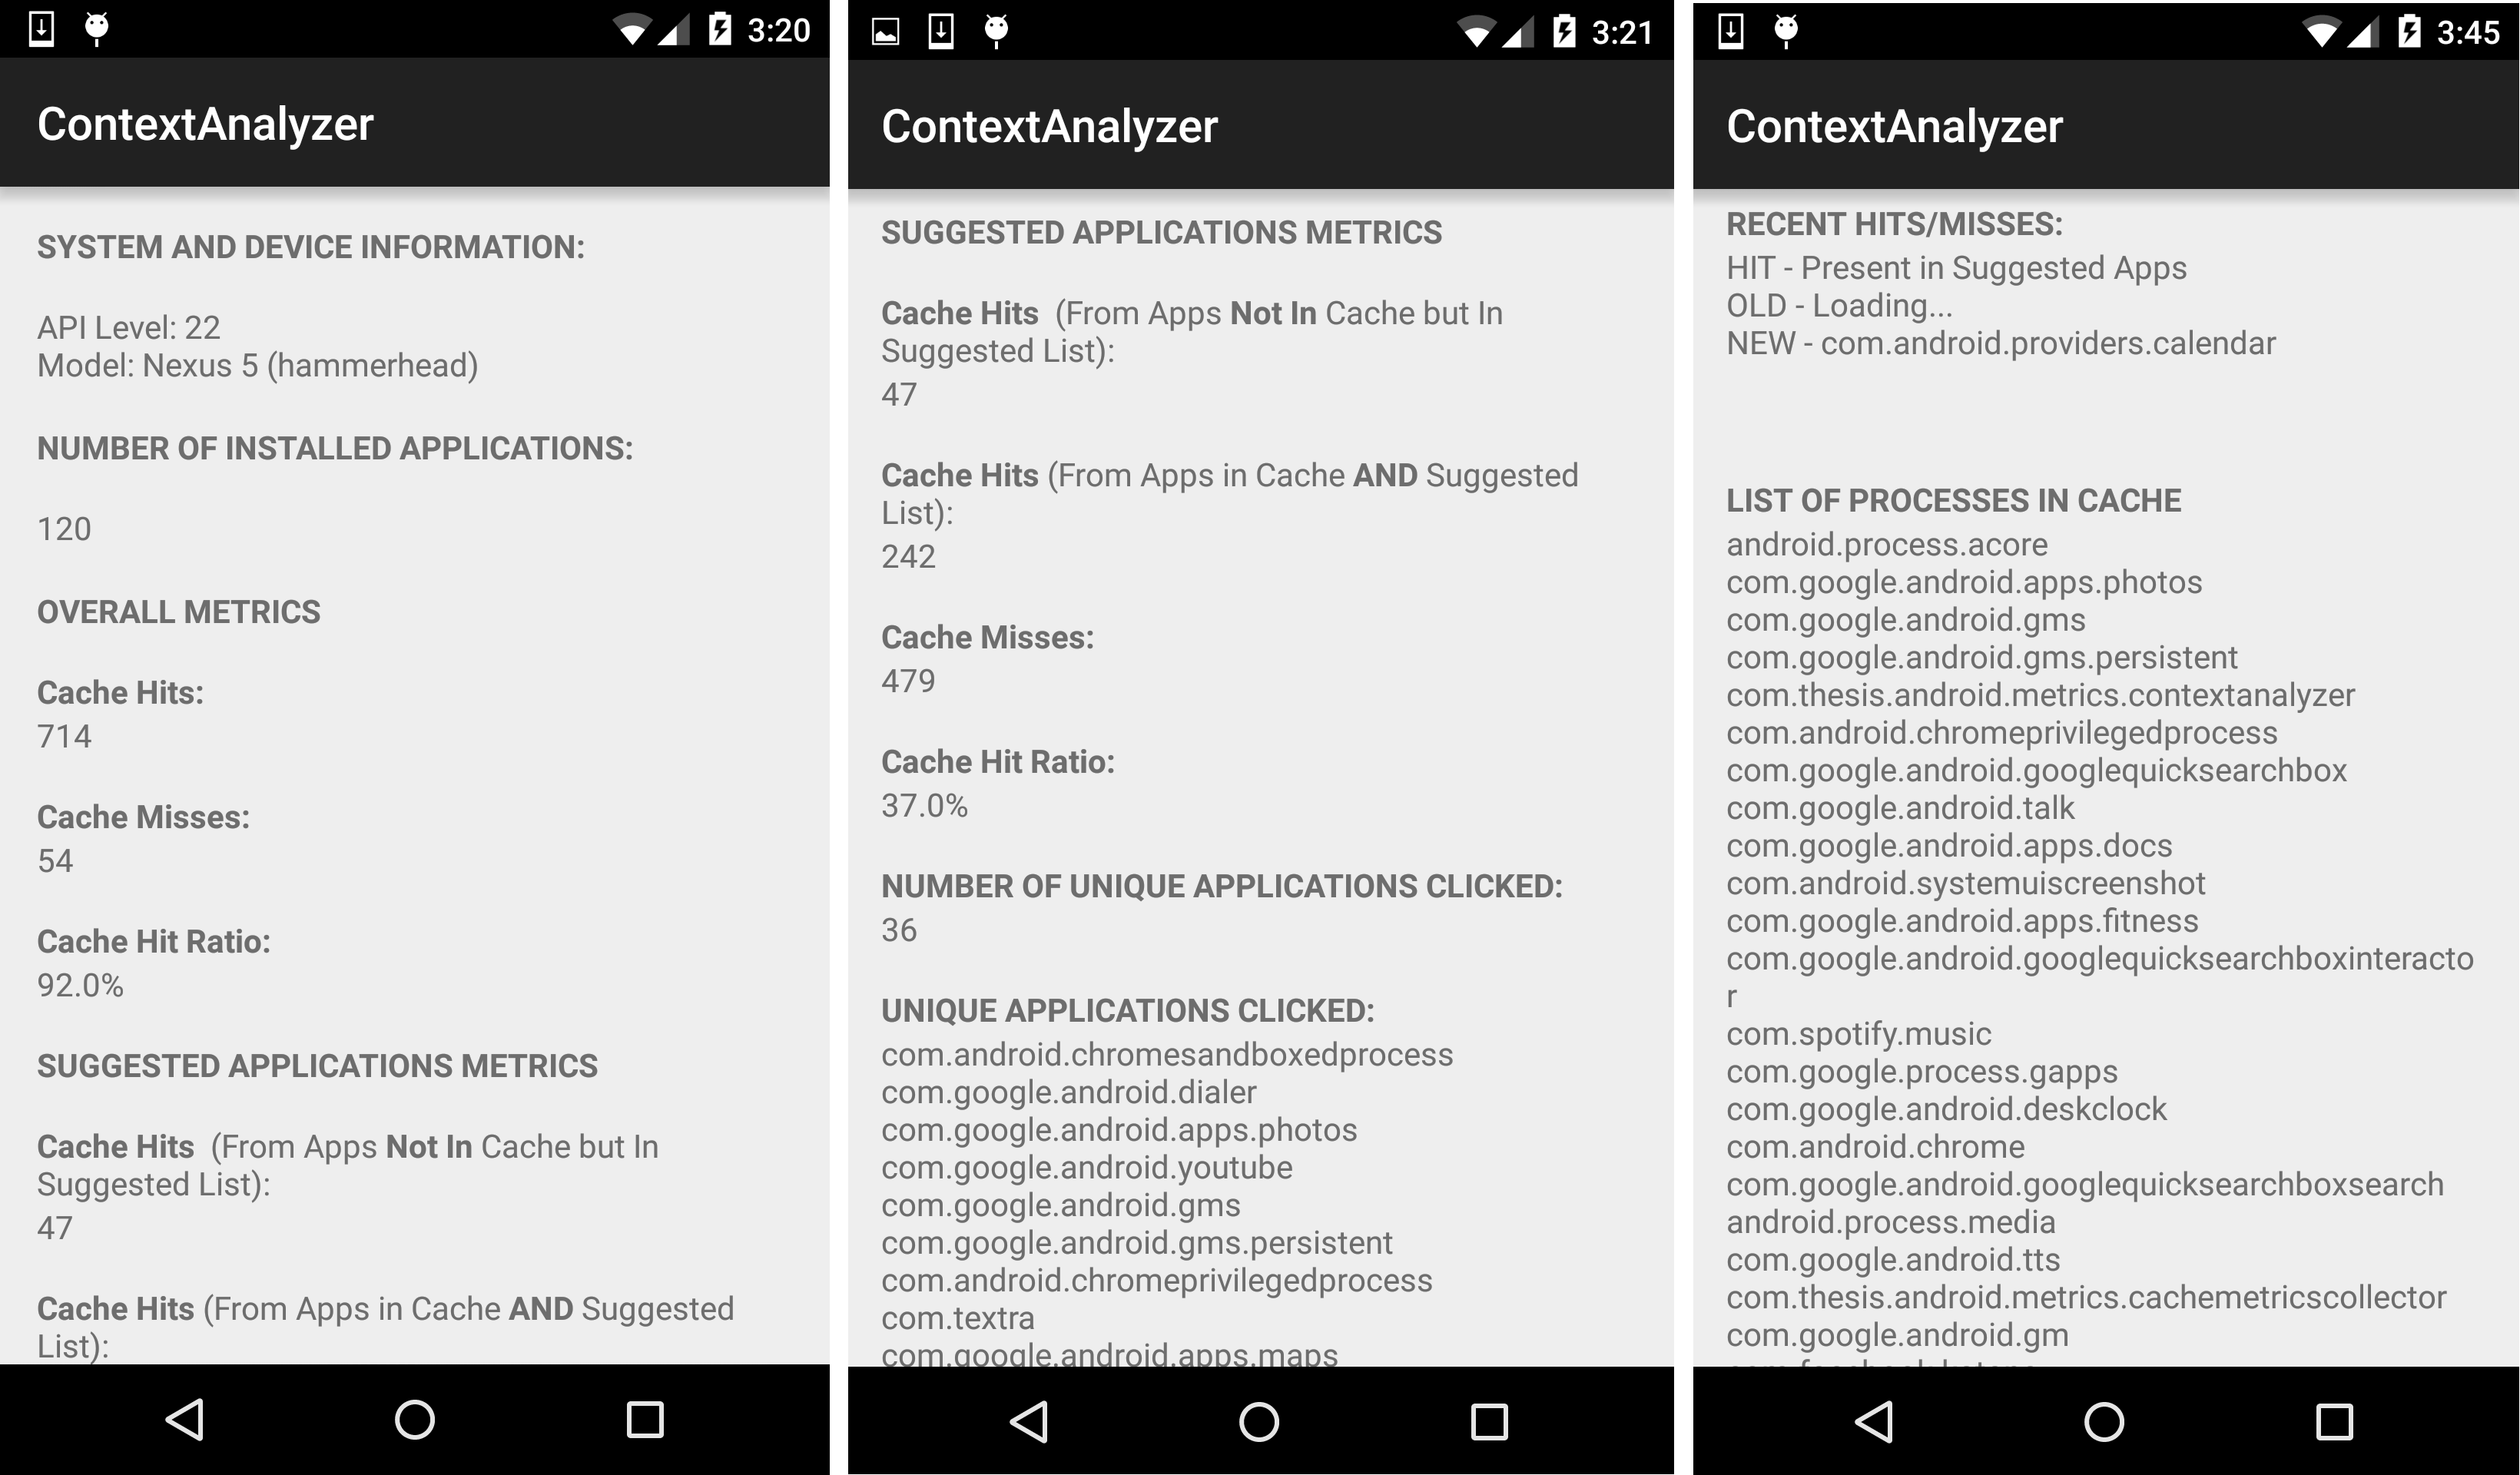
\includegraphics[width = 130mm]{images/contextAnalyzerUI.png}
			\caption[Context Analyzer UI]{The images to the left, middle and right represent the top, middle and bottom portions of the UI respectively. Note that the Cache Hits in the Suggested Applications Metrics section is divided into suggested-exclusive and suggested non-exclusive. In addition to the cache metrics, it also displays some supplementary data such as the number of unique applications clicked, phone model, OS version and the number of installed applications. These details are discussed in Chapter 5 and are presented as demographic data. Finally, it also displays recent cache hits/misses, memory list and the calendar list purely for the user's benefit. It is not used in data analysis in any way.}
		\end{figure}
		
		It is worth noting that {\em ContextAnalyzer} collects sufficient data to compute the CHR of three distinct caching schemes:
		
		\begin{itemize}			
			\item Hybrid Scheme
			\item Pure Prediction Scheme
			\item Default Scheme
		\end{itemize}
		
		Since it collects the overall cache hits and overall cache misses, it is quite straightforward to see how it would compute the CHR of the Hybrid scheme.
		
		\begin{equation}
			Hybrid CHR = \frac{Overall Hits}{Overall Misses}
		\end{equation}
		
		The total hits for the pure prediction approach can be obtained by summing the suggested-exclusive hits and the suggested non-exclusive hits as their total comprises of all the hits that resulted due to the calendar list. The application also collects the suggested misses, therefore the CHR for the pure prediction approach can be easily obtained.
		
		\begin{equation}
			Total Suggested Hits = SuggestedExclusive  Hits + Suggested NonExclusive  Hits			
		\end{equation}
		
		\begin{equation}			
			Pure Prediction CHR = \frac{Total Suggested Hits}{Total Suggested Hits + Suggested Misses}
		\end{equation}
		
		The total hits and misses for the default scheme can be derived from the data that {\em ContextAnalyzer} directly collects. Since it collects the overall cache hits (that includes default cache hits) and the suggested-exclusive cache hits, the default cache hits can be obtained by computing their difference:
		
		\begin{equation}
			Default Hits = Overall Hits - Suggested Exclusive Hits
		\end{equation}
		
		Alternatively, we can obtain the default-exclusive cache hits by computing the difference of the overall misses and the suggested misses. This can then be added to suggested non-exclusive cache hits to obtain the total cache hits for the default scheme.
		
		\begin{equation}
			DefaultExclusive Hits = Suggested Misses - Overall Misses
		\end{equation}
		
		\begin{equation}
			Default Hits = DefaultExclusive Hits + Suggested NonExclusive Hits 
		\end{equation}
		
		Every application click that results in a suggested-exclusive cache hit would by extension, also result in a default cache miss. Additionally, every application click that results in an overall cache miss would also result in a default cache miss. Therefore the sum of these two fields would give us the default cache misses.
		
		\begin{equation}
			Default Cache Misses = Overall Cache Misses + Suggested Exclusive Cache Hits
		\end{equation}
		
		The CHR for the default scheme can be computed using the following equation:
		
		\begin{equation}
			Default Cache Hit Ratio = \frac{Default Cache Hits}{Default Cache Hits + Default Cache Misses}
		\end{equation}
		
		We have established that the application collects sufficient data to compute all the necessary metrics for the three caching schemes. Let us inspect the design of this application. {\em ContextAnalyzer} comprises of the following modules:
		
		\begin{itemize}
			\item Main Activity [1]
			\item Background Service [2]
			\item Process Manager
			\item Calendar Reader
			\item Calendar Parser
		\end{itemize}
		
		The main activity is the heart of the application. It is responsible for launching the application and creating a background service. The background service retrieves the list of processes in memory and the current foreground application. The background service is bound to the activity i.e. it is life-cycle is tied to that of the activity's [36]. It is for this reason that the volunteers are instructed not to forcefully close {\em ContextAnalyzer} for the duration of the experiment as that would destroy the service along with the activity and all metric collection would stop. The process manager module contains a {\em Process} data structure that encapsulates a running process and all of its attributes (name, user identifier, process identifier to list a few). It also contains the algorithm that fetches the list of processes residing in memory. The background service launches a separate thread that invokes this algorithm every second, to compute the cache metrics and update the UI. It also has the additional task of obtaining the calendar list from the calendar parser. The calendar parser gets the list of calendar events from the calendar reader and produces the calendar list (that the service consumes). The calendar reader queries the user's calendar API and obtains the list of events for the next four hours. The following class diagram (Figure 4-2) illustrates {\em ContextAnalyzer}'s design.
	
		\begin{figure}[h]
			\centering
			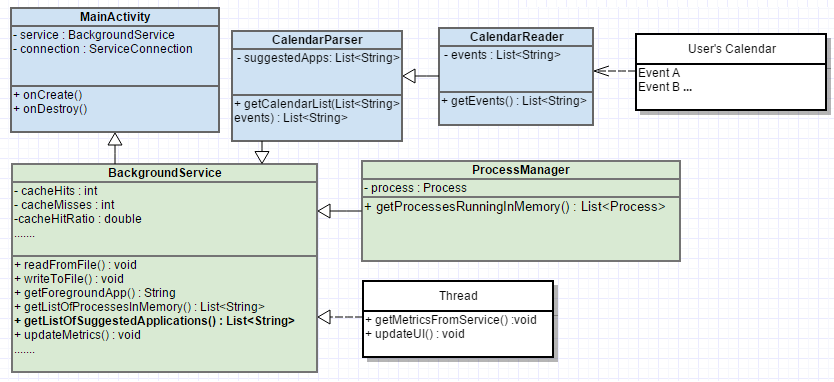
\includegraphics[width = 150mm]{images/contextAnalyzerDesign.png}
			\caption[Context Analyzer Class Diagram]{Context Analyzer Class Diagram}
		\end{figure}
		   

		{\em ContextAnalyzer} was developed using Android Studio [37] and the source code was uploaded on Github [35]. The class diagram was built using Gliffy [38]. The APK file was uploaded on our Github I/O page [39][40].

\chapter{Data Analysis and Results}

		\section{Introduction}
			In Chapter 3, we examined some of the challenges in collecting the data we needed and in the previous chapter, we analyzed {\em ContextAnalyzer}'s design and how the experiment was setup. In this chapter, we will inspect the data we collected from each volunteer and compare the cache hit ratios of each caching scheme (Default, Context \& Default-Context Hybrid). The following section elaborates on the volunteer demographic and the subsequent sections analyze the cache data. Finally, we verify whether our results are statistically significant using a Paired T test [44] and examine the points of weaknesses of this thesis.
			
		\section{Demographic Data}
			Our experiment comprised of twenty volunteers, all of whom were male college students between the ages of nineteen and twenty three. The most common APMD used by the volunteers was the Nexus 5 [45] and SM-G900T (Samsung Galaxy S5) [46] was the least common one. Every volunteer satisfied the Android OS version prerequisite as they all ran Android 5.1 (LOLLIPOP\_MR1) [47]. There were three other metrics  collected from the volunteers that can be classified as demographic data:
			
			\begin{itemize}
				\item Number of Installed Applications (Measured at start of the experiment)
				\item Number of Unique Applications Clicked (During the course of the experiment)
				\item Number of Calendar Entries (During the course of the experiment)
			\end{itemize} 
			
			\subsection{Total Installed Applications}
				The minimum number of installed applications among the volunteers was 120. The maximum number of applications installed by any volunteer was 374. The average number of installed applications was 295. The following chart (Figure 5-1) illustrates this distribution.
				
				\begin{figure}[h]
					\centering
					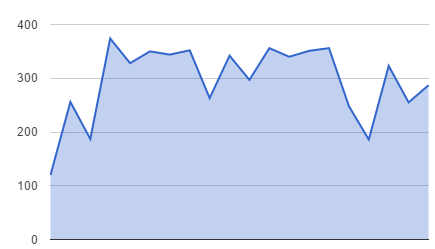
\includegraphics[width = 130mm]{images/totalApps.png}
					\caption[Distribution of Total Installed Applications]{This chart illustrates the distribution for the number of installed applications (measured at the start of the experiment), among the 20 volunteers.}
				\end{figure}
				
			\subsection{Unique Applications Clicked}
				The minimum number of unique applications that were clicked among the volunteers, during the course of the experiment was 34. The maximum number of unique applications requested by any volunteer was 56. The average number of unique applications requested was roughly 46. The following chart (Figure 5-2) illustrates this distribution.
				
				\begin{figure}[h]
					\centering
					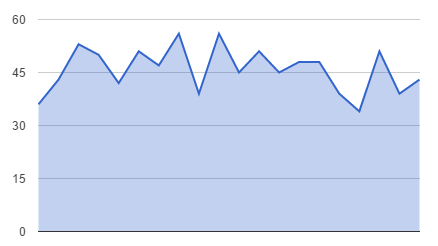
\includegraphics[width = 130mm]{images/uniqueApps.png}
					\caption[Distribution of Unique Applications Requested]{This chart illustrates the distribution for the number of unique applications requested during the course of the experiment, among the 20 volunteers.}
				\end{figure}
				
			\subsection{Calendar Entries}
				The minimum number of calendar entries among the volunteers was 11. The maximum number of entries entered in the calendar by any volunteer was 43. The average number of calendar entries was roughly 25. The following chart (Figure 5-3) illustrates this distribution.
				
				\begin{figure}[h]
					\centering
					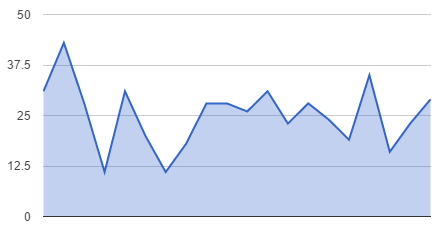
\includegraphics[width = 130mm]{images/calendarEntries.png}
					\caption[Distribution of Number of Calendar Entries]{This chart illustrates the distribution for the number of calendar entries during the course of the experiment, among the 20 volunteers.}
				\end{figure}		
			
			So far, we have analyzed the distribution for the number of installed applications, the number of unique applications clicked and the total number of calendar entries during the course of the experiment. In the next section, we will examine the CHR(s) of each caching scheme and whether there is a correlation between these metrics and the efficiency of certain caching schemes.
			
		\section{Experiment Results}
			The data collected by the {\em ContextAnalyzer} application provides the metrics to measure the efficiencies of three caching schemes (Section 4.4):
			
			\begin{itemize}
				\item Context Scheme
				\item Default Scheme
				\item Default-Context Hybrid Scheme
			\end{itemize}
			
			Let us analyze the data from each scheme. Since the absolute number of cache hits and cache misses vary depending on frequency of smartphone usage, the only relevant metric is the CHR for each scheme. We will examine the CHR(s) in percentages for each caching scheme.
			
			\subsection{Context Scheme}
				The maximum CHR recorded by any volunteer for this scheme was 37.39\%. However, this is not representative of the average case. The mean CHR for the context scheme was 18.47\% with a standard deviation of 7.67\% and a variance of 58.75. The minimum recorded CHR was 5.92\% suggesting that in the worst case, roughly 1 in 16 application requests resulted in a cache hit. The median CHR was 17.35\%. The following box plot (Figure 5-4) illustrates this distribution.
				
				\begin{figure}[h]
					\centering
					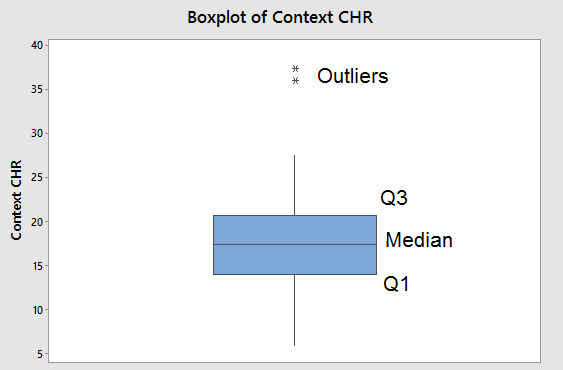
\includegraphics[width = 130mm]{images/contextScheme.png}
					\caption[Distribution of CHR for Context Scheme]{This box plot illustrates the distribution for the CHR(s) in the context scheme, among the 20 volunteers. It is worth noting that 25\% of the volunteers had a CHR of 14.05\% or less i.e. the Q1 value is 14.05\%. Similarly, 75\% of the volunteers had a CHR of 20.68\% or below indicating that the third quartile value or Q3 is 20.68\%. Note that the two outlier values are indicated by the asterisk symbol at the very top. On a side note, this box plot was generated using Minitab, a statistical software package [48].}
				\end{figure}
				
				The average CHR was 18.47\% i.e. roughly 4 in 5 application requests resulted in a cache miss. While it is better than nothing, it remains to be seen whether the default scheme or the default-context hybrid scheme can put up better numbers.	
			
			\subsection{Default Scheme}
				The maximum CHR recorded by any volunteer for this scheme was 93.19\%. However, this is not representative of the average case. The mean CHR for the default scheme was 79.17\% with a standard deviation of 13.87\% and a variance of 192.37. The minimum recorded CHR was 46.52\% suggesting that in the worst case, less than 1 in 2 application requests resulted in a cache hit. The median CHR was 84.04\%. The following box plot (Figure 5-5) illustrates this distribution.
				
				\begin{figure}[h]
					\centering
					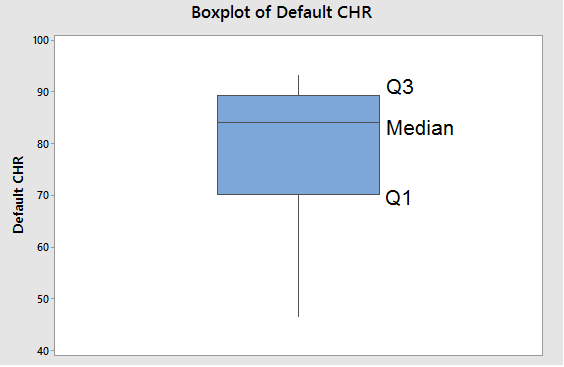
\includegraphics[width = 130mm]{images/defaultScheme.png}
					\caption[Distribution of CHR for Default Scheme]{This box plot illustrates the distribution for the CHR(s) in the default scheme, among the 20 volunteers. It is worth noting that 25\% of the volunteers had a CHR of 70.28\% or less i.e. the Q1 value is 70.28\%. Similarly, 75\% of the volunteers had a CHR of 89.34\% or below indicating that the third quartile value or Q3 is 89.34\%. This box plot was generated using Minitab as well [48].}
				\end{figure}
				
				The average CHR was 79.17\% i.e. roughly 4 in 5 application requests resulted in a cache hit. To put that in perspective, it is more than 4 times the average CHR of the context scheme. Let us see if the hybrid scheme can improve these numbers.
				
			\subsection{Default-Context Hybrid Scheme}
				The maximum CHR recorded by any volunteer for this scheme was 95.62\%. However, this is not representative of the average case. The mean CHR for the hybrid scheme was 83.50\% with a standard deviation of 12.39\% and a variance of 153.49. The minimum recorded CHR was 53.48\% suggesting that in the worst case, less than 1 in 2 application requests resulted in a cache miss. The median CHR was 88.48\%. The following box plot (Figure 5-6) illustrates this distribution.
				
				\begin{figure}[h]
					\centering
					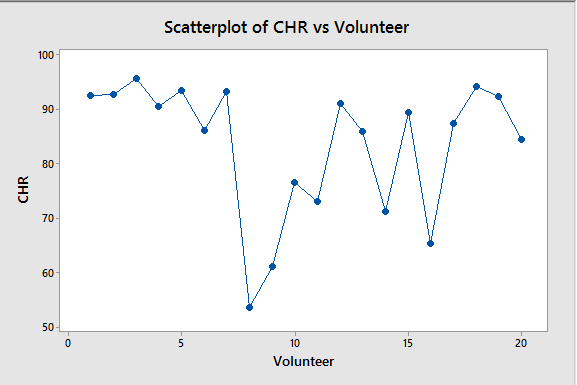
\includegraphics[width = 130mm]{images/hybridScheme.png}
					\caption[Distribution of CHR for Hybrid Scheme]{This box plot illustrates the distribution for the CHR(s) in the hybrid scheme, among the 20 volunteers. It is worth noting that 25\% of the volunteers had a CHR of 73.97\% or less i.e. the Q1 value is 73.97\%. Similarly, 75\% of the volunteers had a CHR of 92.73\% or below indicating that the third quartile value or Q3 is 92.73\%. This box plot was generated using Minitab as well [48].}
				\end{figure}
				
				The average CHR was 83.50\% i.e. roughly more than 4 in 5 application requests resulted in a cache hit. It is worth noting that the hybrid scheme's average CHR is 4.33\% more than that of the default scheme, hinting at an improvement in efficiency. In the next section, we will examine if this increase in CHR is statistically significant, by performing a paired t test [44]. 

		\section{Significance Testing}
			In any experiment or observation that involves drawing a sample from a population, there is always the possibility that an observed effect could have occurred due to sampling error alone [49][50]. In order to prove that the increase in CHR for the hybrid scheme is statistically significant, we performed a paired t test using every [hybrid CHR, default CHR] pair collected over the duration of the experiment (Figures 5-7, 5-8).
			
			\begin{figure}[h]
				\centering
				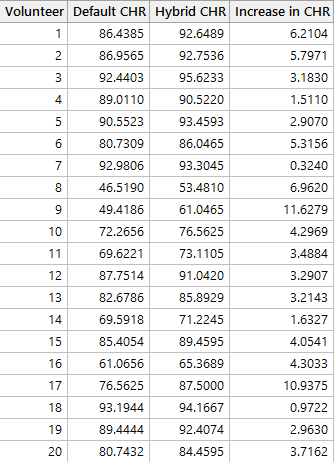
\includegraphics[width = 110mm]{images/chrPairs.png}
				\caption[Relative Increase in CHR - Table]{The data listed in this table illustrates the relative increase in CHR between the default and hybrid schemes for each volunteer. This data is used as the input for the paired t test to measure its statistical significance.}
			\end{figure}
			
			\begin{figure}[h]
				\centering
				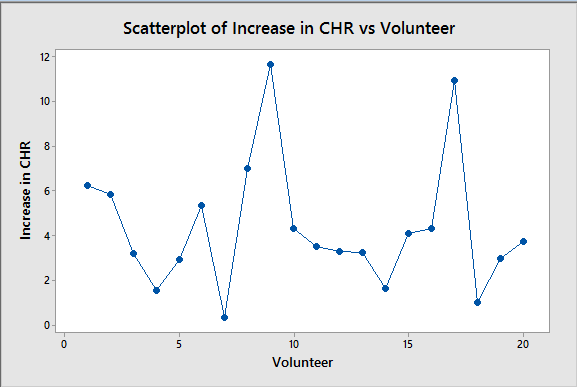
\includegraphics[width = 110mm]{images/chrDifferences.png}
				\caption[Relative Increase in CHR - Chart]{This box plot illustrates the increase in CHR from the default to hybrid scheme for each of the 20 volunteers. Note that the two outliers are indicated by the asterisk symbol at the very top.}
			\end{figure}
			
			Before the test is performed, two things need to be determined:
			\begin{itemize}
				\item Null Hypothesis
				\item Significance Level
			\end{itemize}
			
			The null hypothesis refers to a general statement or a default position that there is no relationship between two measured phenomena [51]. In our case, the null hypothesis would state that there is no difference in the means between the CHR(s) of the default and the hybrid schemes. Our objective is to perform a paired t test and determine the validity of the null hypothesis and by extension the statistical significance of our data. Significance level is the probability of rejecting the null hypothesis given that it is true [52]. By convention, the significance level is set to 0.05 (5\%), implying that it is acceptable to have a 5\% probability of incorrectly rejecting the null hypothesis. The {\em p-value} is defined as the probability of obtaining a result equal to or more statistically extreme than what was actually observed, assuming that the null hypothesis is true [53]. Therefore, if the paired t test produces a p-value less than the significance level i.e. the probability of obtaining more extreme results is less than the probability of incorrectly rejecting the null hypothesis, then the results are statistically significant and the null hypothesis can be rejected. The results of the paired t test are shown in Figure 5-9.
			
			\begin{figure}[h]
				\centering
				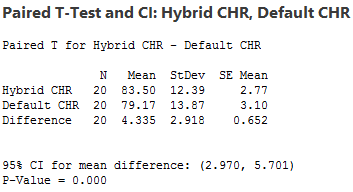
\includegraphics[width = 110mm]{images/pairedTest.png}
				\caption[Paired T Test Resuts]{ This image illustrates the results of a paired t test conducted with the data listed in Figure 5-7. The paired t test was conducted using Minitab [48].}
			\end{figure}			
		
			Given that the {\em p-value} is less than the significance level (0.05), there is strong evidence to reject the null hypothesis. Furthermore, a 95\% CI (Confidence Interval) [54] between 2.97\% \& 5.70\% indicates the lower and upper bound for the true average increase in CHR (If the study were conducted with a larger population). Therefore, it is reasonable to conclude that the increase in CHR between the two caching schemes is not due to sampling error and is statistically significant. In the next section, we will examine potential correlations between the cache hit ratios and some of the demographic data.
			
		\section{Correlation with Demographic Data}
			
			\subsection{Calendar Usage}
				Intuitively, we would expect the increase in CHR to be higher when the calendar usage is higher. Let us examine if such a correlation exists is the data we collected. We compute the PPMCC (Pearson Product Moment Correlation Coefficient) [53] for the increase in CHR and the number of calendar entries for each volunteer (Figure 5-10). 
				
				\begin{figure}[h]
					\centering
					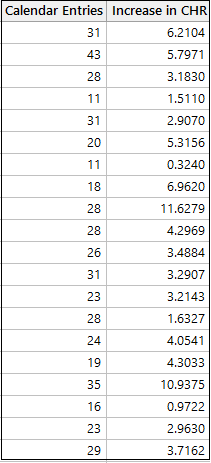
\includegraphics[width = 70mm]{images/calendarData.png}
					\caption[Increase in CHR vs Calendar Entries - Table]{This table illustrates the data used to compute the correlation between increase in CHR and the number of calendar entries entered by each volunteer for the duration of the experiment.}
				\end{figure}
				
				The results of the PPMCC computation (computed using Minitab [48]) were the following:
				
				\begin{itemize}
					\item A PPMCC value of 0.467 
					\item A p-value of 0.038
				\end{itemize}
				
				
				 If we assume the significance level to be 0.05, then a p-value of 0.038 (less than significance level) corroborates the statistical significance of our PPMCC. A PPMCC value of 0.467 signifies a modest positive correlation. Therefore, it is reasonable to conclude that an increase in CHR from the default to hybrid scheme is consistent with an increase in calendar usage among the test subjects. The following fitted line plot (Figure 5-11) illustrates this linear correlation.
				
				 \begin{figure}[h]
				 	\centering
				 	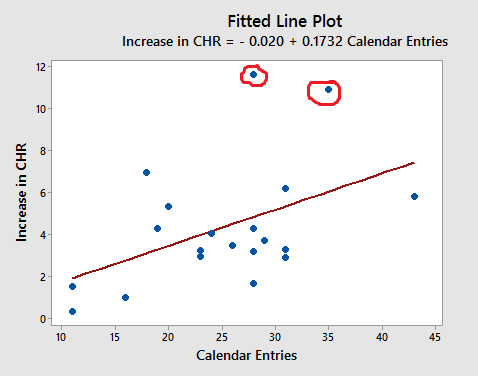
\includegraphics[width = 110mm]{images/regressionPlot.png}
				 	\caption[Increase in CHR vs Calendar Entries - Plot]{This fitted line plot illustrates the linear correlation between increase in CHR and calendar usage. Note that the two outliers are marked at the top with red circles.}
				 \end{figure}
			
			\subsection{Number of Unique Applications Requested}
				
				Let us examine if there is a relationship between the number of unique applications a user requests over the course of the experiment, and an increase in the cache hit ratio. We compute the PPMCC [53] for the increase in CHR and the number of unique applications requested for each volunteer (Figure 5-12). 
				
				\begin{figure}[h]
					\centering
					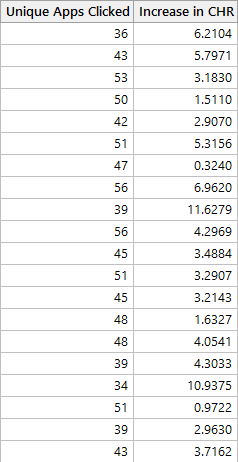
\includegraphics[width = 70mm]{images/uniqueAppsData.png}
					\caption[Increase in CHR vs Unique Applications Requested - Table]{This table illustrates the data used to compute the correlation between increase in CHR and the number of unique applications requested by each volunteer for the duration of the experiment.}
				\end{figure}
				
				 The results of the PPMCC computation (using Minitab [48]) were the following:
				
				\begin{itemize}
					\item A PPMCC value of $-0.437$ 
					\item A p-value of 0.054
				\end{itemize}
				
				
				If we assume the significance level to be 0.05, then a p-value of 0.054 (approximately equal to the significance level) corroborates the statistical significance of our PPMCC. A PPMCC value of $-0.437$ signifies a modest negative correlation. Therefore, it is reasonable to conclude that an increase in CHR from the default to hybrid scheme is consistent with a decrease in the number of unique applications requested among the test subjects. However, it is worth noting that the p-value is within the margin of error compared to a 0.05 significance level. The following fitted line plot (Figure 5-13) illustrates this negative correlation.
				
				\begin{figure}[h]
					\centering
					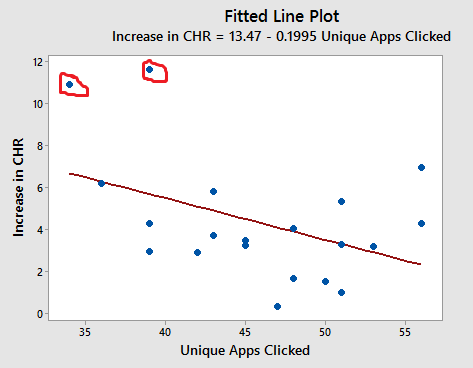
\includegraphics[width = 110mm]{images/uniqueAppsPlot.png}
					\caption[Increase in CHR vs Unique Applications Requested - Plot]{This fitted line plot illustrates the negative correlation between increase in CHR and number of unique applications requested over the course of the experiment. Note that the two outliers are marked at the top with red circles. It is also worth noting that the two highest increases in CHR(s) occurred for the volunteers with the lowest number of unique applications clicked which considerably influenced the result.}
				\end{figure}

\chapter{Points of Weakness}
	While the data demonstrates that incorporating context analysis improves the efficiency of the default caching scheme, there are certain factors that could affect the validity of this thesis:
	
	\begin{itemize}
		\item The volunteers were instructed to use their calendar applications but real-world users may or may not use their calendar application. However, if the users were aware of the benefits in using the calendar under a hybrid scheme, that may change.
		\item The entries in the calendar may not be indicative of the application that the user might use during that calendar event. 
		\item Not all applications can be mapped to keywords obtained from calendar entries. For instance, while {\em call} can be directly mapped to the Caller application, there are no keywords that come to mind for the Camera application.
		\item Since the calendar is only queried every four hours, change in event descriptions within a four hour period are not captured by our application. However, this is merely a design decision and the frequency can be increased to account for this issue. 
		\item If no events were found in the calendar for a four hour period, then the list of suggested applications is set to a default list derived from the most popular Android applications in USA (Section 3.3.7). A significant amount of the cache hits for the hybrid scheme could have occurred as a result of the requested application being found in this default list rather than the applications truly inferred from calendar events.
		\item If the volunteer requests two applications within a span of a second (highly unlikely but theoretically possible), then our application would only count the cache hit/miss from the second request as the thread only checks for a new foreground application every second.
		\item The lack of diversity in our volunteer demographic could have influenced the data. Given that all research volunteers were male college students, the rate of smartphone usage was quite high. It would have been conducive to gather volunteers of all ages and gender.
		\item Due to our policy of full transparency, the volunteers were aware of the type of data being collected. Even though there was no inherent motivation for any of the volunteers to intentionally skew the cache metrics, theoretically they had the ability to do so. 
		\item The volunteers were instructed not to close the application for the duration of the experiment but this was not enforced. Technically, a volunteer could have selectively closed the application for certain times of the day resulting in an inaccurate monitoring period. However, they had no motivation to do so as no personal information was being collected.
	\end{itemize}  		

\chapter{Conclusion}
	The typical user is not facing a desktop machine in the relatively predictable office environment anymore. smartphones are well suited to utilize contextual information in enhancing the behavior of their applications. However, the full potential of context analysis is not harnessed by Android devices. Currently, the Android OS caches application components in memory, based on recency of application usage. We have demonstrated that incorporating context information improves the efficiency of this caching scheme. For this purpose, we set up an experiment comprising of twenty volunteers. We developed an Android application to measure the cache metrics of both the default recency-based caching scheme and a default-context hybrid scheme, which in addition to relying on recency of usage, parsed the user's calendar for contextual clues. We analyzed the data and proved that on an average, the hybrid scheme had a significantly higher cache hit ratio. By virtue of its superior efficiency, the hybrid scheme would result in a lower startup time for relatively more applications, thereby enhancing the overall user experience.
		
\chapter{Future Work}		
	In addition to the user's calendar, other sources of information can be utilized to obtain context. These days, most APMD(s) have built-in sensors that measure motion, orientation, and various environmental conditions. These sensors are capable of providing raw data with high precision and accuracy, and are useful in monitoring three-dimensional device movement or positioning, or changes in the ambient environment near a device [7]. Information from multiple sensors can significantly improve the reliability of contextual data. Shi et al.'s work focused on constructing a user behavior model [8] based on analyzing user behavior. A similar approach can be used to predict the list of applications the user is likely to use in the immediate future. Currently the calendar parser relies on predetermined mapping between keywords and applications. This can me improved upon by learning the user's preferences. If the user predominantly requests an application, associated with a particular event in the calendar, then the mapping can be altered by learning the user's preferences. Finally, this thesis merely verifies whether a caching scheme that incorporates context information is more efficient than the default recency-based scheme. The next step would be to implement this caching scheme by building a custom distribution of the Android OS, facilitated by the AOSP [43].

	
%XXXXXXXXXXXXXXXXXXXXXXXXXXXXXXXXXXXXXXXXXXXXXXXXXXXXXXXXXXXXXXXXXXXX
%XXXXXXXXXXXXXXXXXXXXXXXXXXXXXXXXXXXXXXXXXXXXXXXXXXXXXXXXXXXXXXXXXXXX
%XXXXXXXXXXXXXXXXXXXXXXXXXXXXXXXXXXXXXXXXXXXXXXXXXXXXXXXXXXXXXXXXXXXX
%XXXXXXXXXXXXXXXXXXXXXXXXXXXXXXXXXXXXXXXXXXXXXXXXXXXXXXXXXXXXXXXXXXXX

%--------+----------------------------------------------------------+
%        |  \myreferences{}                          (CONDITIONAL)  |
%        |                                                          |
%        |  See section 3.18 of "Read_Me_First_(v12).pdf"           |
%        |                                                          |
%        |  That section of the READ ME file describes two options  |
%        |  for listing the works cited in your document: first,    |
%        |  manually entering your list of references and, second,  |
%        |  using BibTeX to generate that list.                     |
%        |                                                          |
%        |  1) If you manually enter your reference list, first     |
%        |     include the \myreferences command, as illustrated    |
%        |     below.  Second, use the "referencelist" environment  |
%        |     described below.  For this, note that the UT Manual  |
%        |     requires double-spacing *between* references in      |
%        |     that list. However, it also states that *within*     |
%        |     individual references the spacing may be single- or  |
%        |     double-spaced.  Because of this, UThesis provides    |
%        |     two options for the "referencelist" environment:     |
%        |                                                          |
%        |            \begin{referencelist}{ENTER OPTION HERE}      |
%        |            \item ...                                     |
%        |            \end{referencelist}                           |
%        |                                                          |
%        |     a. Replacing "ENTER OPTION HERE" above with the      |
%        |        text "single" will generate a reference list      |
%        |        with single-spaced entries in that list but       |
%        |        double-spacing between those entries. An example  |
%        |        of this is provided below.                        |
%        |     b. Alternatively, using the "double" option will     |
%        |        generate a list with double-spaced entries and    |
%        |        double-spacing between entries. An example of     |
%        |        this is also provided below.                      |
%        |                                                          |
%        |     Note that input to these options is case sensitive   |
%        |     and the default setting is the "double" option.      |
%        |                                                          |
%        |  2) If you instead choose to use BibTeX to generate the  |
%        |     reference list, then you *cannot* include either     |
%        |     the "\myreferences" command or the "referencelist"   |
%        |     environment in your document. In this case you must  |
%        |                                                          |
%        |     a. delete the \myreferences command and the two      |
%        |        examples of the "referencelist"  environment      |
%        |        below;                                            |
%        |     b. then you must add and locate appropriately all    |
%        |        necessary BibTeX commands within your document    |
%        |        (e.g., \bibliographystyle{}, \citationstyle{},    |
%        |        \bibliography{}, etc.).                           |
%        +----------------------------------------------------------+

\myreferences

\begin{referencelist}{single}

	\item \textbf{[1]} ``Activities | Android Developers''
	\\\emph{http://developer.android.com/guide/components/activities.html}, October 2015. 
	Online; Last Accessed: October 22, 2015.					     

	\item \textbf{[2]} ``Services | Android Developers''
	\\\emph{http://developer.android.com/guide/components/services.html}, October 2015. 
	Online; Last Accessed: October 22, 2015.
	
	\item \textbf{[3]} ``Processes and Application Life Cycle''
	\\\emph{http://developer.android.com/guide/topics/processes/process-lifecycle.html}, October 2015. 
	Online; Last Accessed: October 22, 2015.
		
	\item \textbf{[4]} ``Hannu Verkasalo - Contextual patterns in mobile service usage''
	\\\emph{http://lib.tkk.fi/Diss/2009/isbn9789512298440/isbn9789512298440.pdf}, March 2008. 
	Online; Last Accessed: October 23, 2015.
			
	\item \textbf{[5]} ``Mika Raento, Antti Oulasvirta, Renaud Petit, and Hannu Toivonen - ContextPhone: A Prototyping Platform for Context-Aware Mobile Applications''
	\\\emph{http://dl.acm.org/citation.cfm?id=1070628}, May 2005. 
	Online; Last Accessed: October 23, 2015.
	
	\item \textbf{[6]} ``Anind K.~Dey, Gregory D.~Abowd and Daniel Salber - A Conceptual Framework and a Toolkit for Supporting the Rapid Prototyping of Context-Aware Applications ''
	\\\emph{http://www.cc.gatech.edu/fce/ctk/pubs/HCIJ16.pdf}, January 2001. 
	Online; Last Accessed: October 23, 2015.
	
	\item \textbf{[7]} ``Sensors | Android Developers''
	\\\emph{http://developer.android.com/guide/topics/sensors/sensors\_overview.html}, October 2015. 
	Online; Last Accessed: October 23, 2015.
	
	\item \textbf{[8]} ``Elaine Shi, Yuan Niu, Markus Jakobsson, and Richard Chow - Implicit Authentication through Learning User Behavior''
	\\\emph{markus-jakobsson.com/wp-content/uploads/2010/11/ShiNiuJakobssonChow2010.pdf}, November 2010. 
	Online; Last Accessed: October 23, 2015.

	\item \textbf{[9]} ``Alan Jay Smith - Design of CPU Cache Memories''
	\\\emph{http://www.eecs.berkeley.edu/Pubs/TechRpts/1987/CSD-87-357.pdf}, August 1987. 
	Online; Last Accessed: October 23, 2015.
			
	\item \textbf{[10]} ``Cache Hit | Techopedia''
	\\\emph{https://www.techopedia.com/definition/6306/cache-hit}, October 2015. 
	Online; Last Accessed: October 23, 2015.
	
	\item \textbf{[11]} ``Cache Miss | Techopedia''
	\\\emph{https://www.techopedia.com/definition/6308/cache-miss}, October 2015. 
	Online; Last Accessed: October 23, 2015.	
									
	\item \textbf{[12]} ``Najeeb A. Al-Samarraie - And Page Replacement Algorithms: Anomaly Cases''
	\\\emph{http://www.iasj.net/iasj?func=fulltext\&aId=50712}, January 2003. 
	Online; Last Accessed: October 23, 2015.
										
	\item \textbf{[13]} ``LRU Replacement Policy''
	\\\emph{https://www.seas.upenn.edu/~cit595/cit595s10/handouts/LRUreplacementpolicy.pdf}, October 2015. 
	Online; Last Accessed: October 24, 2015.
	
	\item \textbf{[14]} ``Donghee Lee, Member, IEEE, Jongmoo Choi, Member, IEEE, Jong-Hun Kim, Member, IEEE,
	Sam H. Noh, Member, IEEE, Sang Lyul Min, Member, IEEE, Yookun Cho, Member, IEEE, and
	Chong Sang Kim, Senior Member, IEEE - LRFU: A Spectrum of Policies that
	Subsumes the Least Recently Used and
	Least Frequently Used Policies''
	\\\emph{http://u.cs.biu.ac.il/~wiseman/2os/lru/lrfu.pdf}, December 2001. 
	Online; Last Accessed: October 24, 2015.

	\item \textbf{[15]} ``An Upper Limit For Apps? New Data Suggests Consumers Only Use Around Two Dozen Apps Per Month''
	\\\emph{http://techcrunch.com/2014/07/01/an-upper-limit-for-apps-new-data-suggests-consumers-only-use-around-two-dozen-apps-per-month/}, July 2014. 
	Online; Last Accessed: October 24, 2015.
											
	\item \textbf{[16]} ``ARM Documentation''
	\\\emph{http://infocenter.arm.com/help/index.jsp?topic=/com.arm.doc.set.cortexr/index.html}, July 2014. 
	Online; Last Accessed: October 24, 2015.

	\item \textbf{[17]} ``Does Your Android Device Really Need a Task Killer?''
	\\\emph{http://www.technorms.com/40664/android-task-killer-apps}, September 2014. 
	Online; Last Accessed: October 24, 2015.
											
	\item \textbf{[18]} ``CyanogenMod''
	\\\emph{http://www.cyanogenmod.org/}, October 2015. 
	Online; Last Accessed: October 24, 2015.
											
	\item \textbf{[19]} ``Activity Manager | Android Developers''
	\\\emph{http://developer.android.com/reference/android/app/ActivityManager.html}, October 2015. 
	Online; Last Accessed: October 24, 2015.
	
	\item \textbf{[20]} ``Usage Stats Manager | Android Developers''
	\\\emph{https://developer.android.com/reference/android/app/usage/UsageStatsManager.html}, October 2015. 
	Online; Last Accessed: October 24, 2015.																			

	\item \textbf{[21]} ``Android Debug Bridge | Android Developers''
	\\\emph{http://developer.android.com/tools/help/adb.html}, October 2015. 
	Online; Last Accessed: October 24, 2015.

	\item \textbf{[22]} ``ADB Shell Commands | Android Developers''
	\\\emph{http://developer.android.com/tools/help/shell.html}, October 2015. 
	Online; Last Accessed: October 24, 2015.
	
	\item \textbf{[23]} ``Android Toolbox''
	\\\emph{http://elinux.org/Android\_toolbox}, October 2015. 
	Online; Last Accessed: October 24, 2015.
	
	\item \textbf{[24]} ``Chainfire | Github | libsuperuser''
	\\\emph{https://github.com/Chainfire/libsuperuser}, October 2015. 
	Online; Last Accessed: October 24, 2015.
	
	\item \textbf{[25]} ``Jared Rummler | Github | AndroidProcesses''
	\\\emph{https://github.com/jaredrummler/AndroidProcesses}, October 2015. 
	Online; Last Accessed: October 24, 2015.

	\item \textbf{[26]} ``toolbox | Github''
	\\\emph{https://github.com/android/platform\_system\_core/tree/master/toolbox}, October 2015. 
	Online; Last Accessed: October 24, 2015.	
					
	\item \textbf{[27]} ``Low RAM Configuration | Android Source Code''
	\\\emph{https://source.android.com/devices/tech/config/low-ram.html}, October 2015. 
	Online; Last Accessed: October 24, 2015.
						
	\item \textbf{[28]} ``OOM Killer''
	\\\emph{http://linux-mm.org/OOM\_Killer}, October 2015. 
	Online; Last Accessed: October 24, 2015.
	
	\item \textbf{[29]} ``Storage Options | Android Developers''
	\\\emph{http://developer.android.com/guide/topics/data/data-storage.html}, October 2015. 
	Online; Last Accessed: October 24, 2015.

	\item \textbf{[30]} ``Calendar Provider | Android Developers''
	\\\emph{http://developer.android.com/guide/topics/providers/calendar-provider.html}, October 2015. 
	Online; Last Accessed: October 24, 2015.

	\item \textbf{[31]} ``These are the 25 most popular mobile apps in America''
	\\\emph{http://qz.com/481245/these-are-the-25-most-popular-2015-mobile-apps-in-america/}, August 2015. 
	Online; Last Accessed: October 24, 2015.
	
	\item \textbf{[32]} ``Google Play''
	\\\emph{https://play.google.com/store}, October 2015. 
	Online; Last Accessed: October 24, 2015.
											
	\item \textbf{[33]} ``Package Manager | Android Developers''
	\\\emph{http://developer.android.com/reference/android/content/pm/PackageManager.html}, October 2015. 
	Online; Last Accessed: October 24, 2015.

	\item \textbf{[34]} ``Chapter 4 - Processes''
	\\\emph{http://www.tldp.org/LDP/tlk/kernel/processes.html}, October 2015. 
	Online; Last Accessed: October 24, 2015.
	
	\item \textbf{[35]} ``Context Analyzer | Github''
	\\\emph{https://github.com/Buzz-Lightyear/Context-Analyzer}, October 2015. 
	Online; Last Accessed: October 24, 2015.
	
	\item \textbf{[36]} ``Bound Services | Android Developer Guide''
	\\\emph{http://developer.android.com/guide/components/bound-services.html}, October 2015. 
	Online; Last Accessed: October 24, 2015.	
	
	\item \textbf{[37]} ``Android Studio | Android Developer Guide''
	\\\emph{http://developer.android.com/tools/studio/index.html}, October 2015. 
	Online; Last Accessed: October 24, 2015.
											
	\item \textbf{[38]} ``Gliffy''
	\\\emph{https://www.gliffy.com/}, October 2015. 
	Online; Last Accessed: October 24, 2015.
							
	\item \textbf{[39]} ``Github Pages''
	\\\emph{https://pages.github.com/}, October 2015. 
	Online; Last Accessed: October 24, 2015.
	
	\item \textbf{[40]} ``Buzz-Lightyear Github | Cache-Analyzer-APK''
	\\\emph{http://buzz-lightyear.github.io/Cache-Analyzer-APK/}, October 2015. 
	Online; Last Accessed: October 24, 2015.
	
	\item \textbf{[41]} ``API Level 21 | Android Developers''
	\\\emph{https://developer.android.com/about/versions/android-5.0.html}, October 2015. 
	Online; Last Accessed: October 28, 2015.	
	
	\item \textbf{[42]} ``Google Inc Apps''
	\\\emph{https://play.google.com/store/apps/developer?id=Google+Inc.\&hl=en}, October 2015. 
	Online; Last Accessed: October 28, 2015.
											
	\item \textbf{[43]} ``Android Open Source Project''
	\\\emph{https://source.android.com/}, October 2015. 
	Online; Last Accessed: October 29, 2015.

	\item \textbf{[44]} ``Mathematics Learning Support Center''
	\\\emph{http://www.statstutor.ac.uk/resources/uploaded/paired-t-test.pdf}, October 2015. 
	Online; Last Accessed: October 29, 2015.

	\item \textbf{[45]} ``Nexus 5X | Google''
	\\\emph{https://www.google.com/nexus/5x/}, October 2015. 
	Online; Last Accessed: October 29, 2015.

	\item \textbf{[46]} ``Samsung Galaxy S5''
	\\\emph{http://www.samsung.com/us/support/owners/product/SM-G900TZKATMB}, October 2015. 
	Online; Last Accessed: October 29, 2015.
																		
	\item \textbf{[47]} ``Android 5.1 API(s) | Android Developer''
	\\\emph{https://developer.android.com/about/versions/android-5.1.html}, October 2015. 
	Online; Last Accessed: October 29, 2015.	

	\item \textbf{[48]} ``Minitab''
	\\\emph{https://www.minitab.com/en-us/}, October 2015. 
	Online; Last Accessed: October 29, 2015.				

	\item \textbf{[49]} ``Babbie, Earl R.~, The Logic of Sampling''
	\\\emph{The Practice of Social Research (13th ed.). Pages 185–226}, October 2013.  Last Accessed: October 30, 2015.	
							
	\item \textbf{[50]} ``David, H.~A.~; Gunnink, Jason L, The Paired t Test Under Artificial Pairing''
	\\\emph{The American Statistician 51 (1): 9–12}, March 1997. Last Accessed: October 30, 2015.
	
	\item \textbf{[51]} ``Everitt, Brian, The Cambridge Dictionary of Statistics''
	\\\emph{Cambridge, UK New York: Cambridge University Press}, March 1998. Last Accessed: October 30, 2015.

	\item \textbf{[52]} ``Schlotzhauer, Sandra, Elementary Statistics Using JMP (SAS Press) (1 ed.)''
	\\\emph{Cary, NC: SAS Institute. pp. 166–423}, March 2007. Last Accessed: October 30, 2015.

	\item \textbf{[53]} ``Stigler, Stephen M.~, Francis Galton's Account of the Invention of Correlation''
	\\\emph{ Statistical Science 4 (2): 73–79.}, April 1989. Last Accessed: October 30, 2015.

	\item \textbf{[54]} ``Cox D.~R.~, Hinkley D.~V.~, Theoretical Statistics''
	\\\emph{Chapman \& Hall, p49, p209}, April 1974. Last Accessed: October 30, 2015.					
\end{referencelist}


%XXXXXXXXXXXXXXXXXXXXXXXXXXXXXXXXXXXXXXXXXXXXXXXXXXXXXXXXXXXXXXXXXXXX
%XXXXXXXXXXXXXXXXXXXXXXXXXXXXXXXXXXXXXXXXXXXXXXXXXXXXXXXXXXXXXXXXXXXX
%XXXXXXXXXXXXXXXXXXXXXXXXXXXXXXXXXXXXXXXXXXXXXXXXXXXXXXXXXXXXXXXXXXXX
%XXXXXXXXXXXXXXXXXXXXXXXXXXXXXXXXXXXXXXXXXXXXXXXXXXXXXXXXXXXXXXXXXXXX

%--------+----------------------------------------------------------+
%        |  \appendix                                  (IF NEEDED)  |
%        |                                                          |
%        |  See section 3.19 of "Read_Me_First_(v12).pdf"           |
%        |                                                          |
%        |  1) When you include the \appendix command a subsequent  |
%        |     \chapter{} command will not generate a chapter but   |
%        |     an appendix section.                                 |
%        |                                                          |
%        |  2) As is illustrated below, to generate a second or     |
%        |     third appendix you simply have to include            |
%        |     additional \chapter{} commands (i.e., you DO NOT     |
%        |     have to repeat the use of the \appendix command).    |
%        +----------------------------------------------------------+

%\appendix
%
%\chapter{Insert the Heading to Appendix A}
%
%[Insert text to Appendix A (if appendix is needed)]
%
%%====================================================================
%
%\chapter{Insert the Heading to Appendix B}
%
%[Insert text to Appendix B (if appendix is needed)]

%XXXXXXXXXXXXXXXXXXXXXXXXXXXXXXXXXXXXXXXXXXXXXXXXXXXXXXXXXXXXXXXXXXXX
%XXXXXXXXXXXXXXXXXXXXXXXXXXXXXXXXXXXXXXXXXXXXXXXXXXXXXXXXXXXXXXXXXXXX
%XXXXXXXXXXXXXXXXXXXXXXXXXXXXXXXXXXXXXXXXXXXXXXXXXXXXXXXXXXXXXXXXXXXX
%XXXXXXXXXXXXXXXXXXXXXXXXXXXXXXXXXXXXXXXXXXXXXXXXXXXXXXXXXXXXXXXXXXXX

%--------+----------------------------------------------------------+
%        |  \end{document}                              (REQUIRED)  |
%        |                                                          |
%        |  Details (if you can call them "details") are provided   |
%        |  in section 3.20 of "Read_Me_First_(v12).pdf"            |
%        +----------------------------------------------------------+

\end{document} %---> ---> ---> --->   DO NOT ALTER THIS COMMAND

%XXXXXXXXXXXXXXXXXXXXXXXXXXXXXXXXXXXXXXXXXXXXXXXXXXXXXXXXXXXXXXXXXXXX
%XXXXXXXXXXXXXXXXXXXXXXXXXXXXXXXXXXXXXXXXXXXXXXXXXXXXXXXXXXXXXXXXXXXX
%XXXXXXXXXXXXXXXXXXXXXXXXXXXXXXXXXXXXXXXXXXXXXXXXXXXXXXXXXXXXXXXXXXXX
%XXXXXXXXXXXXXXXXXXXXXXXXXXXXXXXXXXXXXXXXXXXXXXXXXXXXXXXXXXXXXXXXXXXX
